\documentclass[11pt]{article}

% Loaded by main.tex
\usepackage[utf8]{inputenc}
\usepackage[T1]{fontenc}
\usepackage{amsmath,amssymb,amsthm}
\usepackage{booktabs}
\usepackage{graphicx}
\usepackage{xcolor}
\usepackage[margin=1in]{geometry}
\usepackage[hidelinks]{hyperref}
\usepackage{microtype}
\usepackage[numbers,sort&compress]{natbib}
\bibliographystyle{unsrtnat}

\newcommand{\E}{\operatorname{E}}
\newcommand{\Var}{\operatorname{Var}}
\newcommand{\logit}{\operatorname{logit}}

% Repository paths render verbatim and link to the file on GitHub.  Write the
% path with real underscores: \repofile{examples/foo_bar.R}
\newcommand{\repobase}{https://github.com/jeonglab-bcm/BARCS/blob/main}
\newcommand{\repotree}{https://github.com/jeonglab-bcm/BARCS/tree/main}
\newcommand{\repofile}[1]{\href{\repobase/#1}{\nolinkurl{#1}}}
\newcommand{\repodir}[1]{\href{\repotree/#1}{\nolinkurl{#1/}}}
\definecolor{barcsblue}{HTML}{0072B2}
\definecolor{mageckorange}{HTML}{D55E00}
\definecolor{chronosgreen}{HTML}{009E73}
\definecolor{mageckpink}{HTML}{CC79A7}
\definecolor{bagelgold}{HTML}{E69F00}
\definecolor{waterbearpurple}{HTML}{7A3E9D}
\definecolor{maudered}{HTML}{A33D3D}
\definecolor{naivegray}{HTML}{767676}
\definecolor{cbtwocyan}{HTML}{56B4E9}
\newcommand{\methodswatch}[1]{\textcolor{#1}{\rule{1.1ex}{1.1ex}}}
\newtheorem{lemma}{Lemma}
\newtheorem{proposition}{Proposition}
\newtheorem{corollary}{Corollary}


\title{BARCS generalizes beta-binomial CRISPR-screen inference\\
to longitudinal and covariate-adjusted designs}
\author{Hyun-Hwan Jeong}
\date{\today}

\begin{document}

\maketitle

% !TeX root = ../main.tex
\begin{abstract}
\noindent\textbf{Background.}  Beta-binomial models represent a guide count as
a proportion conditional on its library total.  Existing CRISPR implementations
of this idea are largely restricted to two-group comparisons, whereas modern
screens often require time, dose, donor, or interaction effects.

\noindent\textbf{Methods.}  BARCS implements guide-level beta-binomial
regression,
$\logit(\mu_{gi})=\mathbf{x}_i^\top\boldsymbol{\beta}_g$.  It conditions each
guide count on the unfiltered library total, estimates prespecified
coefficients or contrasts, and optionally uses negative-control calibration
and dispersion moderation.  Simulations with known truth and held-out controls
were used to distinguish ranking performance from error-rate calibration.

\noindent\textbf{Results.}  In a correctly specified continuous-dose
simulation, unmoderated BARCS was anti-conservative: its null type-I error was
0.081 and its empirical false-discovery proportion was 0.130 at nominal 0.05,
versus 0.038 and 0.049 for MAGeCK-MLE.  A five-fold held-out analysis of 593
non-targeting guides in an IL2RA screen gave a BARCS $p<0.05$ rate of 0.049
after control scaling, but the correlated FACS-bin design remains outside the
independent-library model.  A Cas13 sensitivity analysis used days 0, 7, and 14
in four replicate-complete cell lines; BARCS had a lower mean
cell-line-specific null calibration
error than MAGeCK-MLE (0.025 versus 0.057), whereas MAGeCK-MLE and general
RNA-sequencing methods ranked essential genes more strongly.  Because these
inputs were normalized, ComBat-corrected, and rounded, that comparison does not
validate either count likelihood.  Dispersion and denominator ablations
improved BARCS in simulations, but they do not establish superiority over
competing methods.

\noindent\textbf{Conclusions.}  BARCS supplies a design-matrix extension of
beta-binomial CRISPR-screen analysis, but the present plug-in dispersion
estimator does not provide uniformly calibrated finite-sample inference.
Independent biological replication, likelihood-compatible counts, and
held-out or cross-fitted controls are required.  The results support the
software contribution and define the work needed for confirmatory use; they do
not show that beta-binomial regression dominates negative-binomial methods.
\end{abstract}


\section{Introduction}
% !TeX root = ../main.tex
Pooled CRISPR screens increasingly measure guide abundance across more than
two experimental conditions.  Examples include time courses, dose series,
ordered FACS fractions, donor-stratified experiments, and factorial designs.
In these studies the scientific estimand is a trend, an adjusted association,
or an interaction.  Reducing the experiment to a high-versus-low comparison
discards intermediate observations and prevents direct adjustment for
additional design variables.

The sampling model is consequential in this setting.  RNA-sequencing methods
typically model a transcript count with a negative-binomial distribution and
represent library size through normalization or an offset
\citep{anders2010deseq,love2014deseq2,law2014voom,lun2016edger}.  Several
CRISPR-screen methods adopted this framework
\citep{li2014mageck,li2015mageckvispr}.  A pooled-guide count also has a known
denominator, however: the total number of mapped guide reads in that library.
Conditional on this total, guide abundance is a proportion.  The
beta-binomial model represents this structure directly and separates
depth-dependent sampling variation from heterogeneity among biological
libraries.  In the original CB\textsuperscript{2} study, goodness-of-fit
comparisons favored the beta-binomial over negative-binomial alternatives for
pooled CRISPR counts \citep{jeong2019beta}.

Beta-binomial regression itself is not new.  The \texttt{corncob} framework
models both the mean and overdispersion of counts conditional on library totals
\citep{martin2020corncob}, and general implementations are available in
\texttt{aod}, \texttt{VGAM}, and \texttt{gamlss}
\citep{lesnoff2012aod,yee1996vgam,rigby2005gamlss}.  BARCS is therefore not
presented as the first beta-binomial regression method.  Its contribution is a
CRISPR-screen implementation that preserves immutable guide-library totals,
uses an R design matrix, returns guide-level coefficient tests at screen scale,
and connects this workflow to CB\textsuperscript{2}.

CB\textsuperscript{2} applies its sampling model to two independent groups.
For guide $g$ observed in library $i$, let $K_{gi}$
denote the guide count, $N_i$ the unfiltered mapped-guide total, and
$\mathbf{x}_i^\top$ one row of a prespecified, full-rank sample design matrix.
The regression problem is
\begin{equation}
  K_{gi}\mid N_i
  \sim \operatorname{BetaBinomial}(N_i,\mu_{gi},\rho_g),
  \qquad
  \logit(\mu_{gi})=\mathbf{x}_i^\top\boldsymbol{\beta}_g,
  \qquad
  H_0:\mathbf{c}^\top\boldsymbol{\beta}_g=0 .
  \label{eq:intro-target}
\end{equation}
Here time, dose, donor, batch, or treatment is a sample-level predictor; the
guide proportion remains the response.  Independent biological libraries,
not individual reads, determine the residual degrees of freedom.

Existing methods address parts of this problem.  Repeated two-group analyses
cannot estimate one coefficient conditional on the remaining columns of the
design matrix.  General RNA-sequencing tools support arbitrary designs but do
not condition each guide on its observed library total.  At the other end of
the spectrum, Chronos and Waterbear model population dynamics or joint FACS-bin
membership, respectively, but are tied to those experimental structures
\citep{dempster2021chronos,pimentel2024waterbear}.  A general-purpose,
depth-aware coefficient test for pooled CRISPR designs remains missing.

We introduce BARCS (Beta-binomial Analysis and Regression for CRISPR Screens)
to fill this gap.  BARCS retains the beta-binomial sampling principle of
CB\textsuperscript{2}, replaces the two group means with an R model matrix, and
tests a prespecified coefficient or contrast with sample-level inference.  The
relationship to CB\textsuperscript{2} is structural: both methods condition
guide counts on library totals and cap the information contributed by deeper
sequencing.  Their estimators, effect scales, dispersion assumptions, and
finite-sample reference distributions differ, so BARCS is not claimed to nest
the implemented CB\textsuperscript{2} test.

The empirical evaluation begins with calibration under known truth.  It then
uses the three-time-point Cas13 study of four replicate-complete cell lines from
\citet{liang2026lncrna} as a processed-count sensitivity analysis and an
ordered-bin IL2RA screen as a held-out-control diagnostic.  Genome-scale and
factorial simulations examine dispersion moderation and denominator choice.
The serially harvested HT-29 culture, endpoint screens, and copy-number
analyses are retained as descriptive robustness checks rather than evidence for
sample-level longitudinal inference.

This design supports a deliberately limited claim.  BARCS makes a
library-total-conditional beta-binomial mean model available to designs that
CB\textsuperscript{2} cannot represent.  Whether its coefficient probabilities
are calibrated is a separate empirical question.  The benchmarks therefore
report failures as well as successes and do not treat the sampling-model choice
as proof of superiority over negative-binomial regression.


\section{Results}
% !TeX root = ../main.tex
We first define the specific extension beyond CB\textsuperscript{2}, then test
that extension in longitudinal Cas13 and donor-adjusted IL2RA screens.
Simulations isolate the contributions of dispersion moderation and denominator
choice, and an external audit examines how preprocessing changes apparent
false-discovery behavior.  Endpoint, serial-harvest, copy-number, and
multi-condition follow-up analyses are reported in the Supplement.

% !TeX root = ../main.tex
% Results subsections, in narrative order.
% !TeX root = ../../main.tex
\subsection{Finite-sample calibration is not guaranteed by the sampling model}
\label{sec:calibration}

The first analysis uses known truth rather than biological proxy labels.  We
simulated 200 genes with three guides per gene under the fitted beta-binomial
model, including 160 null genes, 27 independent libraries, a continuous dose,
and three batches.  The tested model therefore matches the data-generating mean
and variance families.  Gene probabilities use the prespecified directional
Stouffer summary for BARCS and the native gene statistic for MAGeCK-MLE.

\begin{table}[htbp]
\centering
\caption{Nominal-versus-realized error rates in the continuous-dose
beta-binomial simulation.  Type-I error is the fraction of 160 null genes with
$p<0.05$.  Empirical FDP is measured among calls at Benjamini--Hochberg FDR
0.05.  This single deterministic simulation is a diagnostic, not a claim of
uniform operating characteristics.}
\label{tab:type1}
\small
\setlength{\tabcolsep}{5pt}
\begin{tabular}{lrrrr}
\toprule
Method & Null type I & Power & Calls & Empirical FDP\\
\midrule
Naive binomial $z$ & 0.844 & 1.000 & 174 & 0.770\\
BARCS unmoderated $t$ & 0.081 & 1.000 & 46 & 0.130\\
BARCS moderated $t$ & 0.088 & 1.000 & 44 & 0.091\\
Official MAGeCK-MLE Wald & 0.038 & 0.975 & 41 & 0.049\\
\bottomrule
\end{tabular}
\end{table}

BARCS is anti-conservative in this example despite correct beta-binomial
simulation.  The guide-level null rate is 0.077, so the failure is already
present before gene aggregation.  No fitted guide reaches the lower
$\widehat\rho=0$ boundary; the truncation mechanism is therefore not the cause
in this simulation.  More generally, the model-based covariance treats
$\widehat\rho$ as fixed, and the residual-$t$ reference does not propagate
guide-specific dispersion uncertainty.  Moderation lowers the empirical FDP
but does not restore nominal type-I error.

Negative controls can diagnose this behavior, but evaluation must be separated
from estimation.  In the IL2RA FACS screen, 0.133 of 593 non-targeting guides
have raw $p<0.05$.  The tail-quantile calibration sets its scale from the
control tail, so measuring those same controls after calibration would be
circular.  Five-fold cross-fitting instead estimates each scale on four folds
and scores the omitted fold.  The resulting held-out rate is 0.049.  This is a
valid out-of-sample diagnostic of the scaling rule at the selected threshold;
it does not repair the correlation among bins from one donor or validate the
independent-library likelihood.

The processed Liang analysis provides a secondary, weaker diagnostic.  BARCS
has a macro-averaged null $p<0.05$ rate of 0.064.  Its reported calibration
error, 0.025, is the mean of the four cell-line-specific absolute errors, not
$|0.064-0.05|=0.014$.  MAGeCK-MLE has corresponding values 0.107 and 0.057.
Because the common matrix was normalized, ComBat-corrected, and rounded before
either fit, these values compare procedures on that transformed input but
cannot establish calibration of their count likelihoods.

% !TeX root = ../../main.tex
\subsection{Longitudinal HT-29 screening}

The first question is whether a continuous predictor observed at more than two
values costs anything relative to methods built for that setting.  We use the
HT-29 time course of
\citet{tzelepis2016dropout}, the longitudinal dataset used to evaluate
Chronos \citep{dempster2021chronos}.  It contains a pDNA measurement and HT-29
guide counts at days 7, 10, 13, 16, 19, 22, and 25.
The three sequencing columns at each late day were summed before analysis.
This distinction is important for the requested $t$ inference: three assays of
one harvested population increase read depth but are not three independent
biological units and therefore must not add residual degrees of freedom.
Following the Chronos preprocessing, guides with fewer than 30 pDNA reads were
removed, leaving 86,882 guides targeting 17,995 genes.

The BARCS and official MAGeCK-MLE 0.5.9.5 fits received the same
eight-column count matrix and the same numeric design, with an intercept and
$d_i/25$.  This is a direct continuous-time comparison.  We also downloaded
the all-seven-time-point Chronos joint result and the deposited per-endpoint
MAGeCK and BAGEL2 results from the Chronos Figshare record
\citep{chronosfigshare2021}.  Those matrices carry one column per day; we use
the day-25 column itself rather than a summary across days, so the comparator
is a single observed endpoint analysis at the deepest time point.

For an external biological target, core essential genes are positives and
HT-29 genes with DepMap 20Q2 expression below 0.5 are negatives, matching the
deposited Chronos analysis.  All methods were
restricted to the same 1,080 essential and 5,774 unexpressed genes.
Null-normalized median difference (NNMD) follows the definition used for
Chronos: the difference between the medians of the two control sets, divided by
the median absolute deviation of the unexpressed effects
\citep{dempster2021chronos}.  No scaling constant is applied, and more negative
values indicate stronger separation.
``False positives'' counts unexpressed genes in the lowest 15\% of all
evaluated effects, following the deposited Chronos analysis.

\begin{table}[ht]
\centering
\caption{Longitudinal HT-29 control-gene benchmark, restricted to the three
methods that fit the full time course.  Deposited single-endpoint results are
reported in the copy-number audit below.  PR AUC is the area under the
precision--recall curve; Recall$_{90}$ is the maximum recall at least 90\%
precision.  Higher AUROC, PR AUC, and Recall$_{90}$ are better; more negative
NNMD and fewer unexpressed false positives are better.  No column maximum is
highlighted, because the differences among these three methods are within the
margins discussed in the text.}
\label{tab:chronos}
\small
\setlength{\tabcolsep}{4pt}
\begin{tabular}{lrrrrr}
\toprule
Method & AUROC & PR AUC & NNMD & Recall$_{90}$ & FP$_{15\%}$\\
\midrule
\methodswatch{barcsblue} BARCS time & 0.9786 & 0.9494 & $-16.34$ & 0.9037 & 74\\
\methodswatch{mageckorange} Official MAGeCK time & 0.9789 & 0.9534 & $-17.75$ &
  0.8972 & 76\\
\methodswatch{chronosgreen} Chronos joint & 0.9747 & 0.9356 & $-27.88$ &
  0.8991 & 77\\
\bottomrule
\end{tabular}
\end{table}

Table~\ref{tab:chronos} does not support declaring a winner.  Continuous-time
MAGeCK has the highest AUROC and PR AUC, BARCS the highest high-precision
recall and the fewest unexpressed false positives, and Chronos by far the
strongest distributional separation.  Every margin except the last is slight:
0.0004 of AUROC, 0.0040 of PR AUC, seven genes of recall out of 1,080, and two
false positives, all from a single run without a resampling interval.  We
therefore do not claim the recall or false-positive column as a BARCS
advantage.  The defensible reading is parity in essential-gene discrimination,
and the claim this benchmark supports is correspondingly modest: a
general-purpose coefficient model gives up nothing here to two methods built
specifically for longitudinal screens.

The deposited single-endpoint results carry a separate caution about analysis
contracts.  Summarising the same deposited MAGeCK matrix by its median across
the seven days rather than by its day-25 column moves its AUROC from 0.9792 to
0.9742 and its recall at 90\% precision from 0.9120 to 0.8602, a swing larger
than any difference among the three models above.  Because early harvests carry
little depletion, an across-day median attenuates the signal the screen was run
to measure.  How a multi-endpoint result is reduced to one number can therefore
matter more than which count model produced it, and the day-25 column is used
wherever those deposited effects appear below.

Chronos's NNMD margin is the one difference in Table~\ref{tab:chronos} that is
not slight, and it is consistent with its mechanistic treatment of knockout
efficiency and saturation.  It should be read as a statement about the shape of
its effect distribution rather than about discrimination: NNMD is the only
metric reported here that is not invariant to monotone rescaling of gene scores
\citep{dempster2021chronos}, and Chronos leads it while trailing both
rank-based metrics.  The BARCS and official continuous-time
MAGeCK effects have Spearman correlation 0.926; correlations with Chronos
joint and the deposited day-25 MAGeCK effects are 0.815 and 0.859.  These are again effect
agreement statistics, not comparable likelihoods: the methods estimate
differently scaled quantities and do not expose a common predictive
likelihood in the deposited outputs.

\clearpage

\subsubsection{What the longitudinal screen says about CNV correction}

We extracted the HT-29 profile (ACH-000552) from DepMap Public 20Q2
\citep{depmap20q2} and repeated the same copy-number audit used for A375.
Before correction, effect--copy-number Spearman correlation among unexpressed
genes is already small: $-0.072$ for BARCS, $-0.075$ for official
continuous-time MAGeCK, $-0.048$ for deposited Chronos joint effects,
$-0.057$ for the published day-25 MAGeCK effects, and $+0.029$ for the
published day-25 BAGEL2 effects.  The BAGEL2 association is the smallest in
absolute value, but that is a narrow robustness observation rather than evidence
of a better classifier: on the same control-gene universe its AUROC is 0.9698,
the lowest of any method examined here.
Applying MAGeCK 0.5.9.5's official piecewise normalizer makes the association
larger in absolute value rather than smaller: $-0.145$ for BARCS and $-0.149$ for
MAGeCK.  Thus the A375 result does not generalize automatically.

This failure mode is informative.  The piecewise correction estimates one
global effect--CNV trend across genes in one cell line and applies it after
model fitting.  When the nuisance association is weak and biological
dependencies are not exchangeable across copy-number regions, the fitted
trend can have the wrong practical target and over-correct null genes.
Chronos joint is shown without CNV correction because the published Chronos
procedure requires multiple cell lines to identify common essential genes and
was explicitly not applied to this single-line experiment
\citep{dempster2021chronos}.  The DepMap profile was measured separately from
the original screen, so cell-line drift is an additional limitation; the
result supports diagnosing correction rather than applying it by default.

% !TeX root = ../../main.tex
\subsection{Longitudinal Cas13 reanalysis separates ranking from calibration}
\label{sec:liang}

The Cas13 fitness screens of \citet{liang2026lncrna} provide a stringent test
of whether the CB\textsuperscript{2} sampling model can support a genuinely
longitudinal design.  We analysed all deposited measurements from days 0, 7,
and 14 in five cell lines.  BARCS, MAGeCK-MLE, edgeR-QL, DESeq2, and
limma--voom estimated the same continuous time slope.  Replicate was included
when complete trajectories were available; K562 lacked one day-0 replicate
and was fitted without the replicate block.  The longitudinal regression
methods used two-sided significance tests.

The deposited values had already undergone median-of-ratios normalization,
ComBat correction, and replicate-outlier processing.  We rounded them once to
the nearest pseudo-count and supplied the same matrix to every method.
Accordingly, this is a processed-count sensitivity analysis rather than a
raw-count likelihood comparison.

Using the intermediate day improved BARCS average precision from 0.776 to
0.786 and recall at gene FDR 0.10 from 0.487 to 0.580 relative to the
two-endpoint fit.  Against longitudinal MAGeCK-MLE, BARCS substantially
improved null calibration: mean absolute calibration error was 0.035 versus
0.103, with average precision 0.786 versus 0.833.  The three general RNA-seq
models had mean null $p<0.05$ rates of 0.139--0.153, compared with 0.076 for
BARCS.

The paired cell-line comparison shows why this difference matters.  BARCS had
the lowest mean absolute calibration error, 0.035, compared with
0.093--0.107 for the alternative longitudinal regression models, while
essential-gene recall at the same empirical 5\% null false-positive rate
remained comparable (0.820 versus 0.840--0.853).  The largest calibration
gains occurred in K562 and MDA-MB-231, where the alternative null rates were
22.4--33.9\% and 14.0--20.0\%, respectively.
Figure~\ref{fig:liang} first shows the complete longitudinal volcano plot for
each method across all five cell lines.  Panels A--C then show three
prespecified-null guide examples for which calibrated BARCS returned
$p=0.20$--$0.23$, while DESeq2, edgeR-QL, and limma--voom each returned
$p<0.05$.  Their library-normalized guide-count trajectories retain both
replicates at each available day, making the longitudinal evidence directly
visible.  These are false-positive calls under the benchmark's prespecified
null definition, not additional biological discoveries.

\begin{figure}[htbp]
\centering
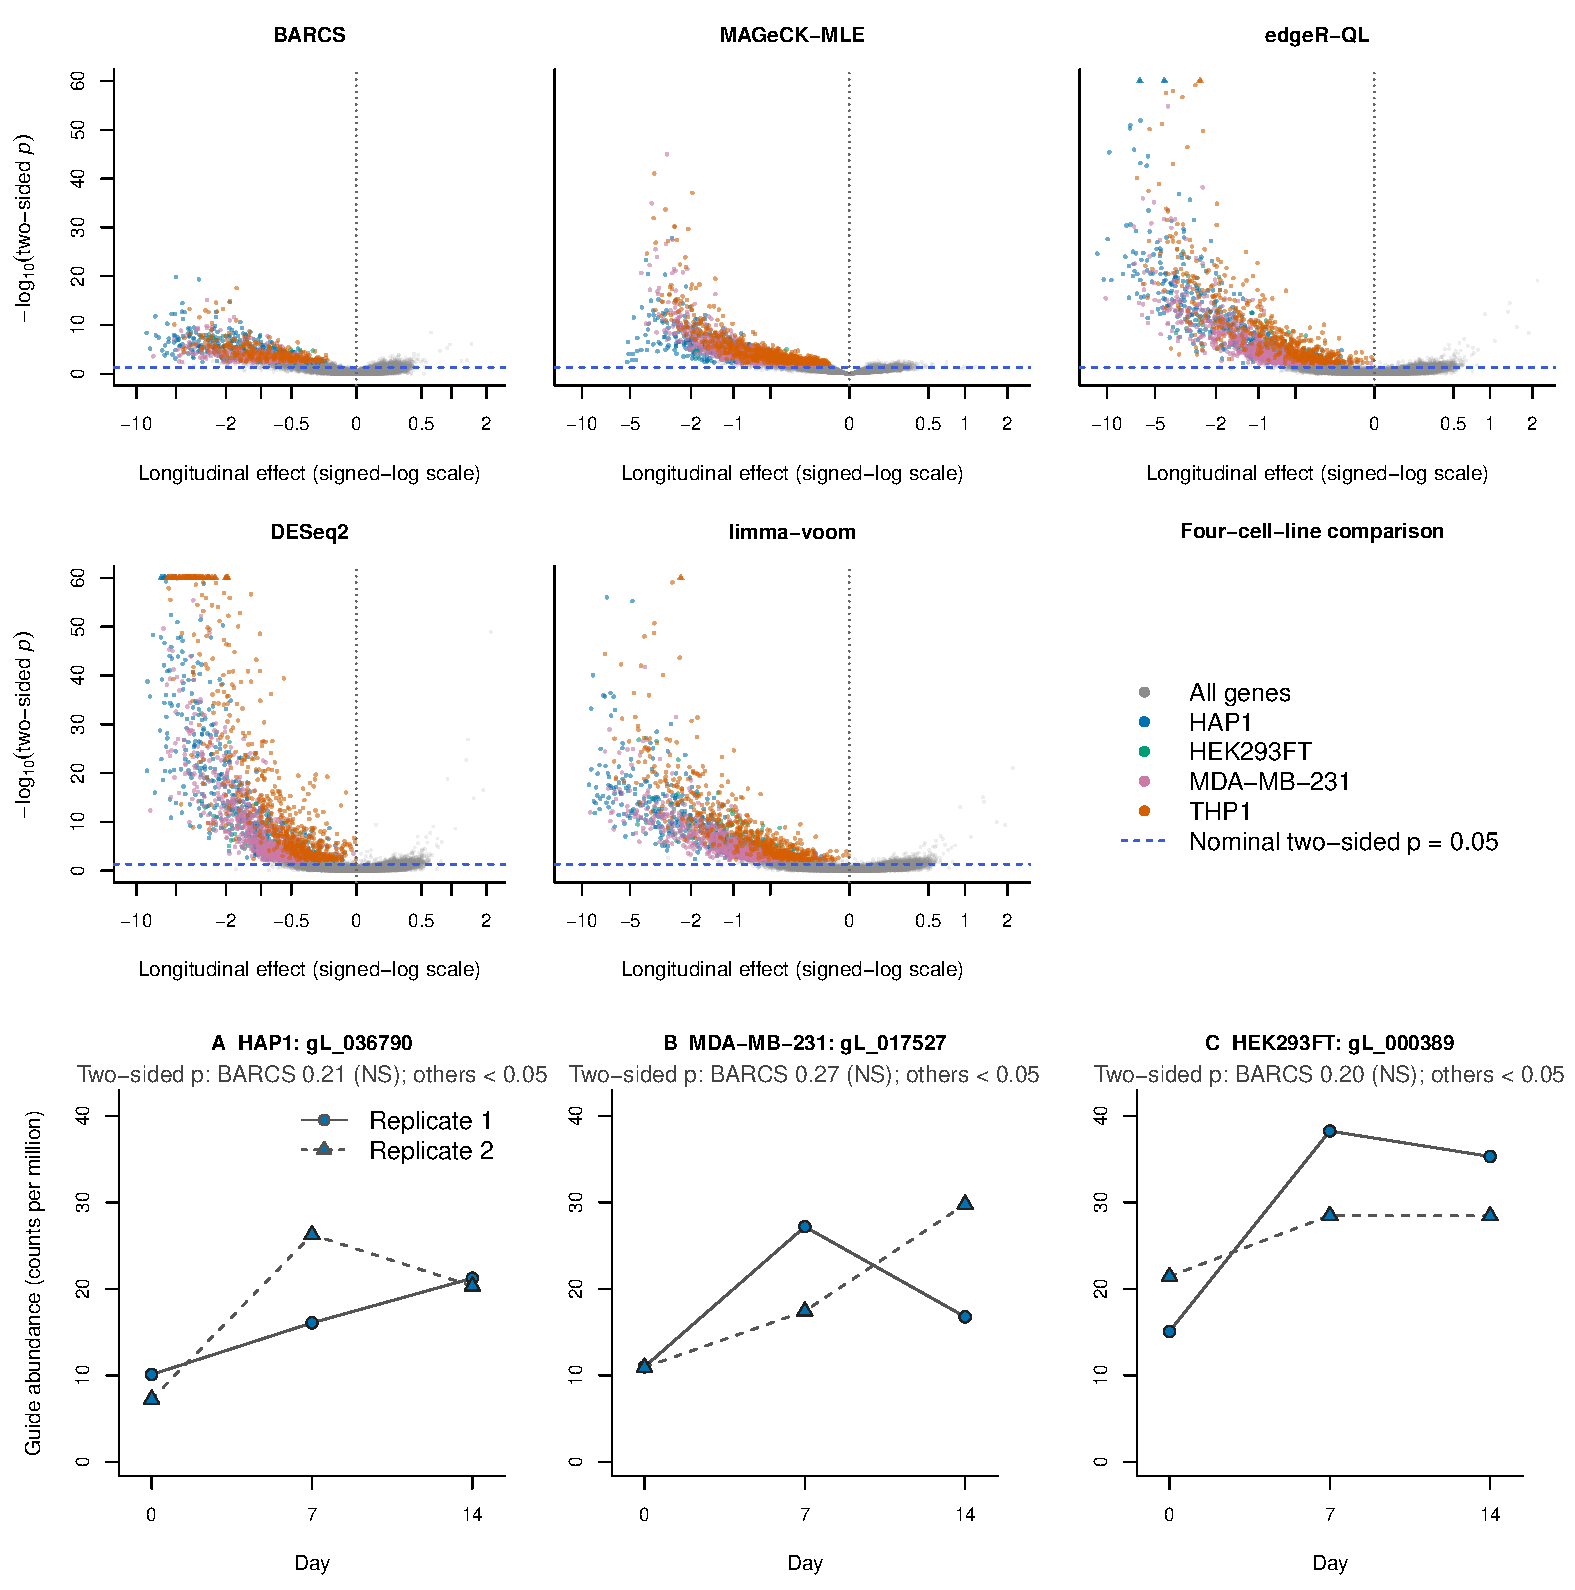
\includegraphics[width=\textwidth]{figures/liang_longitudinal_volcano_trajectories.pdf}
\caption{Longitudinal Cas13 comparison using days 0, 7, and 14.  The upper
rows show method-specific volcano plots for BARCS, MAGeCK-MLE, edgeR-QL,
DESeq2, and limma--voom, pooling gene-level results from HAP1, HEK293FT, K562,
MDA-MB-231, and THP1.  Within each cell line, every method estimates the same
continuous time slope from the identical processed-count matrix.  Colored
points are negatively directed genes called at two-sided FDR 0.10, with color
denoting cell line; the dashed horizontal line marks nominal two-sided
$p=0.05$, and triangles identify $-\log_{10}(p)$ values clipped at 60.
(A--C) Processed
guide counts divided by the corresponding library size, in counts per
million, for three prespecified-null examples.  Lines connect measurements
from the same replicate across days.  BARCS leaves each guide non-significant,
whereas DESeq2, edgeR-QL, and limma--voom each call it significant.
MAGeCK-MLE is included in the gene-level volcano comparison but not in panels
A--C because its reported statistic is gene-level.}
\label{fig:liang}
\end{figure}

Rounding changed each deposited value by less than 0.5, but the upstream
transformations mean that none of the fitted likelihoods retains its literal
raw-count interpretation.  Confirmation from raw reads therefore remains
necessary.  The supplied streaming workflow performs the full longitudinal
preparation for that validation.

% !TeX root = ../../main.tex
\subsection{Stress test and model boundary: ordered-bin FACS}

The Waterbear study supplies a complementary continuous-phenotype benchmark
with unusually useful validation \citep{pimentel2024waterbear}.  GSE242880
contains a pooled CRISPR screen of IL2RA protein abundance in primary human
T cells, from the regulatory-network study of \citet{freimer2022il2ra}, which
is also the source of the individually validated regulators used below.  Its low-coverage, high-MOI arm has four ordered FACS bins for each
of three donors, 6,000 guides targeting 1,350 genes or negative controls, and
26 regulators whose direction was confirmed by individual knockout and flow
cytometry.  Because these are primary donor cells rather than a cancer cell
line, this benchmark is not driven by tumor copy-number artifacts.

We assigned the four bins latent marker locations equal to the conditional
means of standard-normal intervals with the prespecified bin masses
$(0.2,0.3,0.3,0.2)$.  Beta-binomial regression used all 12 libraries with a
marker slope and donor indicators.  Official MAGeCK-MLE received the same
model space; its marker score was affinely mapped to zero--one because the
MAGeCK initializer requires a reference row with all non-intercept entries
zero.  We also fitted two outer-bin ablations and ran the paper's native
\texttt{mageck test} comparison of Q1 with Q4.

This design exposes a limitation of applying independent-library regression
to sorted data.  The four bins from one donor partition one cell pool and are
therefore negatively correlated, while the beta-binomial fit treats their
margins separately.  Among 593 non-targeting guides, the raw all-bin
beta-binomial $p<0.05$ frequency is 0.133.  We therefore added the
prespecified negative-control calibration implemented by
\texttt{bb\_calibrate\_controls()}: the empirical 95th percentile of absolute
control $t$ statistics is matched to the $t_8$ two-sided 0.05 cutoff, with
scales below one prohibited.  The estimated scale is 1.357; after calibration,
the non-targeting frequency is 0.049.  Estimates and the $t$ reference are
retained, while raw and calibrated inferential columns are both saved.

\begin{table}[ht]
\centering
\caption{GSE242880 low-coverage, high-MOI IL2RA FACS benchmark.  Recovery
uses each method's reported 0.10 discovery threshold and the independently
validated direction.  BARCS and MAGeCK use adjusted
$p$-values; Waterbear uses posterior inclusion probability above 0.90.
The non-targeting column is guide-level.  Waterbear and MAUDE values are
reported by the study and were not rerun.  The highest validated recovery and
the available non-targeting rate closest to 0.05 are highlighted.}
\label{tab:waterbear}
\small
\setlength{\tabcolsep}{4pt}
\begin{tabular}{lrrr}
\toprule
Method & Discoveries & Validated recovery & NTC $p<0.05$\\
\midrule
\methodswatch{barcsblue} BARCS, four bins + controls &
  49 & 22/26 & \textcolor{barcsblue}{\textbf{0.049}}\\
\methodswatch{barcsblue} BARCS, four bins raw & 127 & 23/26 & 0.133\\
\methodswatch{mageckorange} Official MAGeCK-MLE, four bins &
  72 & 17/26 & ---\\
\methodswatch{barcsblue} BARCS, outer bins & 34 & 18/26 & 0.064\\
\methodswatch{mageckorange} Official MAGeCK test, outer bins &
  32 & 18/26 & ---\\
\methodswatch{waterbearpurple} Waterbear, four bins (reported) &
  79 & 24/26 & ---\\
\methodswatch{maudered} MAUDE, four bins (reported) &
  406 & \textcolor{maudered}{\textbf{25/26}} & ---\\
\bottomrule
\end{tabular}
\end{table}

The calibrated four-bin BARCS result recovers four more
validated regulators than all-bin MAGeCK-MLE while making 23 fewer calls.  It
is two regulators behind the reported Waterbear result and three behind MAUDE.
The raw 23/26 BARCS result is not the primary claim because
its negative controls reveal inflation.  MAUDE's 25/26 recovery is also not
evidence of superior specificity: it calls 406 of 1,350 genes, and the
Waterbear study found poor MAUDE calibration in simulations
\citep{pimentel2024waterbear,deboer2020maude}.  Across all 1,350 genes,
uncalibrated BARCS and MAGeCK-MLE all-bin effects have
Spearman correlation 0.917, so the recovery difference is not caused by
globally incompatible directions.  All 26 validation effects have the
expected sign under each independently rerun method.

The follow-up table contains more information than the 26-positive subset.
Thirty-three candidates were tested individually: 26 had a concordant IL2RA
effect and seven did not validate.  Restricting evaluation to these measured
labels avoids the incorrect assumption that every other screen gene is a false
positive.  Table~\ref{tab:waterbearpanel} reports threshold and ranking metrics
for the five methods rerun here.

\begin{table}[ht]
\centering
\caption{Classification in the selected 33-gene experimental follow-up panel
(26 concordant positives and seven non-validating candidates).  This panel is
small and was selected from a previous screen, so the metrics are supporting
evidence rather than unbiased genome-wide performance estimates.  Higher is
better for every metric; column maxima are highlighted.}
\label{tab:waterbearpanel}
\small
\setlength{\tabcolsep}{4pt}
\begin{tabular}{lrrrrr}
\toprule
Method & F1 & MCC & Balanced accuracy & AUROC & Avg. precision\\
\midrule
\methodswatch{barcsblue} BARCS, four bins + controls
  & \textcolor{barcsblue}{\textbf{0.863}}
  & \textcolor{barcsblue}{\textbf{0.398}}
  & \textcolor{barcsblue}{\textbf{0.709}} & 0.808 & 0.945\\
\methodswatch{barcsblue} BARCS, four bins raw
  & 0.852 & 0.194 & 0.585
  & \textcolor{barcsblue}{\textbf{0.819}}
  & \textcolor{barcsblue}{\textbf{0.950}}\\
\methodswatch{mageckorange} Official MAGeCK-MLE, four bins
  & 0.723 & 0.070 & 0.541 & 0.626 & 0.872\\
\methodswatch{barcsblue} BARCS, outer bins
  & 0.783 & 0.340 & 0.703 & 0.714 & 0.913\\
\methodswatch{mageckorange} Official MAGeCK test, outer bins
  & 0.766 & 0.224 & 0.632 & 0.703 & 0.906\\
\bottomrule
\end{tabular}
\end{table}

The raw four-bin model has the strongest rank metrics, which indicates that the
continuous trend is extracting useful signal.  Control calibration changes the
decision boundary rather than the estimated effects and produces the best F1,
Matthews correlation, and balanced accuracy in the validation panel.  That
combination is the central evidence for BARCS here:
continuous-bin ranking gains are retained while explicit null guides prevent
the extra calls from being mistaken for confidence.

This benchmark is stronger than a rank-correlation-only comparison because it
contains directionally validated biology and hundreds of explicit null
guides.  It is not an unbiased precision experiment: the 26 genes were chosen
for follow-up from an earlier screen, and unvalidated genes cannot simply be
called false positives.  Nor does it overturn Waterbear's modeling advantage.
Waterbear represents the joint multinomial bin structure, uncertain cutoffs,
guide-to-gene hierarchy, and sparse effects; BARCS supplies
a much faster transparent trend test but needs negative controls here to
diagnose and scale inference under a violated independence assumption.  The deposited paper reports
24/26 for Waterbear and 17/26 for MAGeCK; the independent current
\texttt{mageck test} rerun gives 18/26, a one-gene implementation-level
difference.

These results separate three meanings of ``better.''  First, ranking quality
asks whether validated regulators move toward the top; the raw four-bin model
performs strongly by AUROC and average precision.  Second, decision quality
asks whether a prespecified threshold balances recovery and false calls; the
control-calibrated model leads the rerun methods by F1 and Matthews
correlation.  Third, likelihood fidelity asks whether the sampling dependence
is represented; Waterbear wins that design question because it models all bins
from a donor jointly.  The case for BARCS here rests on its performance on the first two questions
using a simple general-purpose model, together with the control diagnostic that
exposes the third.

\paragraph{MAUDE's own control calibration.}
MAUDE's reported 25/26 recovery is the highest in Table~\ref{tab:waterbear}, and
the non-targeting column is empty for it, so we measured that directly.  MAUDE
consumes non-targeting guides to build its empirical null, which means its
calibration cannot be read off the same guides it was given: those scores are
centred by construction, and all 593 return $p>0.2$.  We therefore split the
control set, declared half to MAUDE as its negative control, and relabelled the
other half so that each held-out guide is scored as its own element.  A held-out
non-targeting guide has no effect, so the rate at which it is called measures the
realised error rate against the nominal one.

Across 891 held-out control tests MAUDE runs at roughly twice its nominal rate
at every threshold: observed 0.021 at a nominal 0.01, 0.095 at 0.05, 0.190 at
0.10, and 0.377 at 0.20, for ratios of 2.13, 1.91, 1.90 and 1.89.  This
reproduces on experimental controls the poor MAUDE calibration that the
Waterbear study reported from simulation \citep{pimentel2024waterbear}, and it
places the 406 calls and 25/26 recovery in context: the recovery is real, and so
is the error rate that buys it.

One scope limit matters here.  MAUDE requires an unsorted reference sample, and
the low-coverage, high-MOI arm analysed above provides only the four sorted
bins, so this calibration was measured on the high-coverage, high-MOI arm, which
deposits a GFP unsorted sample per donor.  It is therefore not the same arm as
the BARCS figure of 0.049 and the two should not be subtracted; what transfers
between arms is the direction and magnitude of the inflation, not the digit.

The published Waterbear and MAUDE aggregates cannot be assigned validation-
panel F1 or Matthews correlation without their gene-level calls for all seven
non-validating candidates.  Reporting 24/26 or 25/26 as if it were complete
accuracy would therefore mix sensitivity with an unknown precision.  We retain
those values as positive-control recovery references and restrict
classification metrics to the methods rerun from complete outputs.

\begin{figure}[ht]
\centering
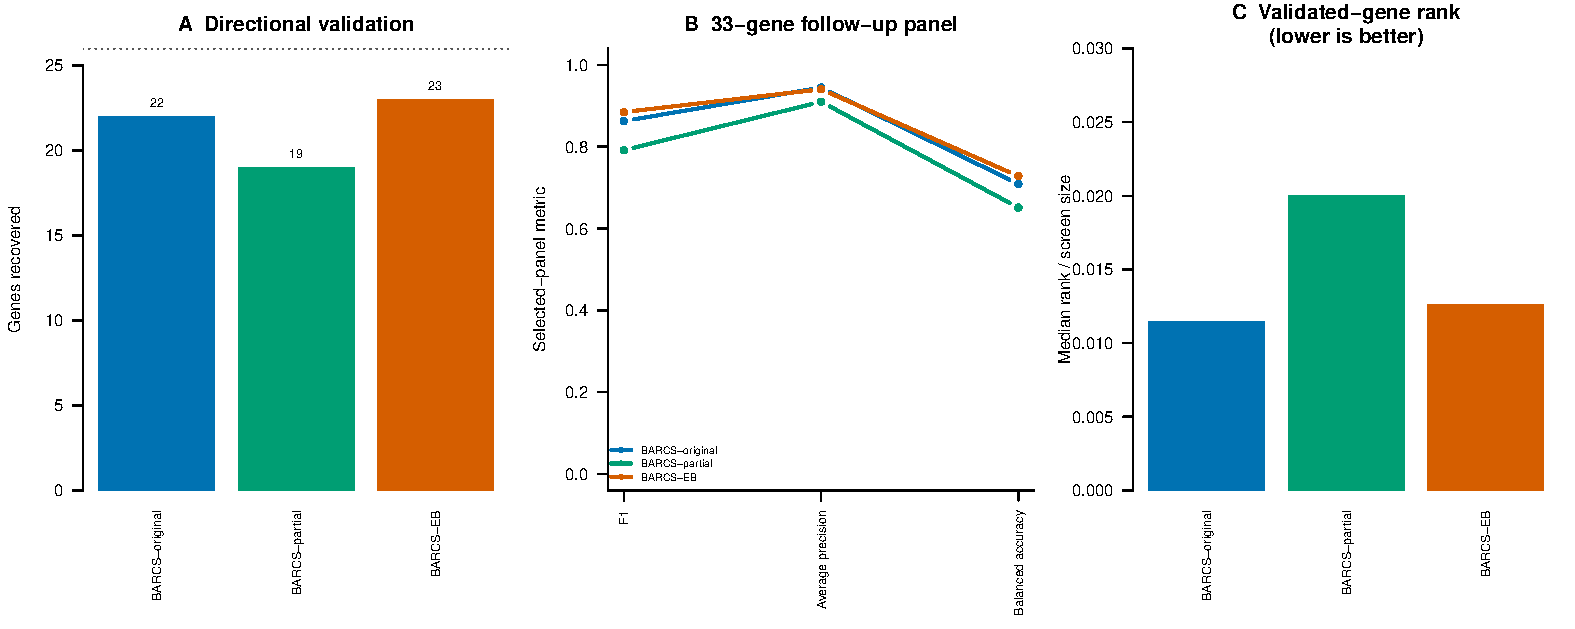
\includegraphics[width=\textwidth]{figures/waterbear_facs_benchmark.pdf}
\caption{Ordered-bin IL2RA FACS benchmark.  (A) Positive-control recovery for
all methods.  (B) F1 in the selected 33-gene panel for methods rerun here.
(C) All-bin BARCS and MAGeCK-MLE effects, with validated genes highlighted.
(D) Non-targeting-guide empirical null curves, showing the correction of raw
all-bin inflation.}
\label{fig:waterbear}
\end{figure}
\clearpage

% !TeX root = ../../main.tex
\subsection{Genome-scale FACS simulation: the effect of dispersion moderation
on the calibration--power tradeoff}

To isolate the FACS design and estimation questions from the
candidate-selected Waterbear validation set, we used CRISPulator 0.5.1
\citep{nagy2017crispulator} to simulate CRISPR knockout screens with known
gene effects at genome scale.  Each of three prespecified seeds generated
10,000 genes, five guides per gene, and four independent screen replicates,
for 50,000 guides per screen.  Twenty percent of genes changed the latent
phenotype and 5\% were explicit negative controls.  The stress-test setting
used phenotype noise $\sigma=2$, 50 sorted cells per guide, and 50 reads per
guide per sample.  Multiplicity of infection was 0.20 in the main analysis
and 0.30 in the supplementary analysis: 0.20 is the operating point at which
the single-integration approximation shared by all of these guide-level
models is most defensible, and 0.30 stresses it.

Each replicate produced a low 0--25\% tail, a high 75--100\% tail, and an
unsorted 0--100\% bulk sample.  The two tails were assigned the conditional
standard-normal locations $-1.271$ and $1.271$; bulk was assigned zero.
Replicate indicators were included in every fit.  We compared this
three-sample fit with the two-tail ablation.  Importantly, ``three sample''
does not mean three independent bins: the bulk sample contains the cell
populations from both tails and costs 50\% more sequencing than the tail-only
design.

Two BARCS gene statistics are carried here.  BARCS-ST
(\texttt{BARCS-original}) is the historical calibrated signed-$z$ statistic.
BARCS-MOD (\texttt{BARCS-moderated}) reuses the same guide fits after
guide-dispersion moderation, which shrinks each guide's variance inflation
toward a library-wide trend before the same signed-$z$ aggregation.  At
genome scale the moderation prior is estimated from 50,000 guides and is
correspondingly sharp: the fitted prior degrees of freedom were 42.7--45.8
against the seven residual degrees of freedom the design itself supplies.

The comparators are the two CRISPR-specific gene callers, MAGeCK-MLE and
CRISPhieRmix \citep{daley2018crisphiermix}, because that is the choice a
screen analyst faces.  They reach the gene level by different routes:
MAGeCK-MLE fits the same design matrix and permutes for its gene FDR, whereas
CRISPhieRmix fits a hierarchical mixture over the guides within a gene, using
the negative-control guides as its empirical null.  It takes guide-level
log$_2$ fold changes, supplied here by a DESeq2 Wald fit of the same design as
its documentation specifies, so DESeq2 enters as a preprocessing step and is
not itself scored.  CRISPhieRmix is run with its bimodal alternative, since
this screen moves the phenotype in both directions and the one-sided default
would score only one of them.

\begin{table}[ht]
\centering
\caption{Genome-scale CRISPulator FACS benchmark at MOI 0.20, 10,000 genes
and 50,000 guides, over three fixed simulation seeds (mean $\pm$ standard
deviation).  All methods are scored on the genes every method returned a
finite result for (9,475--9,517 per run); MAGeCK-MLE omits negative-control
genes from its gene summary once their sgRNAs are declared and CRISPhieRmix
consumes them as its null, so the common set excludes them.  Recall counts
active genes called at gene FDR 0.10 with the
correct direction.  FDP is the realized fraction of inactive genes among
calls; the nominal target is 0.10.  Column maxima for ranking, effect
recovery, recall, and F1 are highlighted.}
\label{tab:crispulator}
\small
\setlength{\tabcolsep}{3pt}
\resizebox{\textwidth}{!}{%
\begin{tabular}{llrrrrrr}
\toprule
Method & Samples & AUROC & Avg.\ precision & Effect $\rho_s$ &
Directional recall & FDP & F1\\
\midrule
\methodswatch{barcsblue} BARCS-ST & Low--bulk--high &
0.947$\pm$.004 & 0.902$\pm$.007 & 0.924$\pm$.004 &
0.716$\pm$.022 & 0.065$\pm$.006 & 0.811$\pm$.012\\
\methodswatch{mageckorange} BARCS-MOD & Low--bulk--high &
0.954$\pm$.003 & 0.919$\pm$.005 & 0.924$\pm$.004 &
0.774$\pm$.014 & 0.066$\pm$.002 &
\textcolor{mageckorange}{\textbf{0.847$\pm$.008}}\\
\methodswatch{naivegray} MAGeCK-MLE & Low--bulk--high &
\textcolor{black}{\textbf{0.957$\pm$.002}} &
\textcolor{black}{\textbf{0.921$\pm$.003}} &
\textcolor{black}{\textbf{0.933$\pm$.002}} &
0.563$\pm$.030 & 0.006$\pm$.002 & 0.718$\pm$.024\\
\methodswatch{chronosgreen} CRISPhieRmix & Low--bulk--high &
0.929$\pm$.004 & 0.867$\pm$.003 & 0.919$\pm$.003 &
0.769$\pm$.025 & 0.197$\pm$.045 & 0.785$\pm$.011\\
\midrule
\methodswatch{barcsblue} BARCS-ST & Low--high &
0.941$\pm$.004 & 0.887$\pm$.008 & 0.923$\pm$.004 &
0.615$\pm$.013 & 0.041$\pm$.001 & 0.749$\pm$.010\\
\methodswatch{mageckorange} BARCS-MOD & Low--high &
0.955$\pm$.003 & 0.920$\pm$.004 & 0.923$\pm$.004 &
0.776$\pm$.012 & 0.063$\pm$.003 & 0.849$\pm$.006\\
\bottomrule
\end{tabular}
}
\end{table}

The two CRISPR-specific comparators fail in opposite directions, and
BARCS-MOD lies between them.  MAGeCK-MLE is the best ranker: it leads AUROC,
average precision, and effect recovery.  CRISPhieRmix is the weakest ranker,
trailing BARCS-MOD by 0.026 AUROC and 0.052 average precision, both intervals
excluding zero.  BARCS-MOD leads F1, and it is the only method here that
combines competitive ranking with a realized FDP below the nominal target.

MAGeCK-MLE converts almost none of its ranking into calls at gene FDR 0.10.
Its realized FDP is 0.006, sixteen times below the 0.10 it was allowed, and
its directional recall is 0.563 against 0.774 for BARCS-MOD.  Paired over the
three seeds its average-precision advantage over BARCS-MOD is 0.0024 (95\%
interval $-0.0029$ to $0.0077$, not resolvable at MOI 0.20), while its F1
deficit is 0.129 ($-0.180$ to $-0.078$).  Its calls are therefore accurate but
highly conservative.  CRISPhieRmix exhibits the converse behavior.  Its
directional recall is statistically indistinguishable from that of BARCS-MOD,
the paired difference being $-0.005$ ($-0.088$ to $+0.078$) and the only such
equivalence in this table, but it attains that recall at realized FDP 0.197
against 0.066, a paired excess of 0.131 (0.018 to 0.245).  Equivalent recall
obtained at three times the error rate is not an equivalent result, and the F1
difference of 0.062 ($0.053$ to $0.071$) quantifies the distinction.

BARCS-MOD therefore attains the operating point that the threshold is intended
to deliver.  It uses most of the permitted false-discovery budget without
exceeding it, 0.066 against the nominal 0.10, and converts this into the
highest F1 among the methods compared.  Neither comparator can be scored on the
negative-control diagnostic, on which BARCS-MOD attains 0.053: MAGeCK-MLE omits negative-control
genes from its gene summary once their sgRNAs are declared, and CRISPhieRmix
consumes them as its empirical null.  That shared omission is also why the
common gene set here is 9,475--9,517 rather than 10,000.

The gain over the historical statistic is unambiguous and is a gain in
ranking rather than a threshold effect: average precision rises from 0.902 to
0.919, a paired difference of 0.017 (0.011 to 0.022), and F1 from 0.811 to
0.847, with realized FDP statistically unchanged.  This is the expected
consequence of estimating the moderation prior from 50,000 guides: a guide
whose own seven residual degrees of freedom understate its variance is
corrected individually, so the negative-control calibration no longer has to
answer those guides with one penalty applied to the whole screen.

Bulk does not supply a new directional contrast.  Across seeds, the
low--bulk--high and tail-only gene effects have mean Spearman correlation
above 0.998.  For the historical statistic its practical contribution is to
the fitted baseline, dispersion, and residual degrees of freedom: mean
directional recall rises from 0.615 to 0.716 and F1 from 0.749 to 0.811, at
50\% more reads.  Moderation largely removes that dependence.  BARCS-MOD
reaches F1 0.849 on the two tails alone against 0.847 with bulk added, so the
information the bulk sample was supplying to the variance model is recovered
more cheaply by borrowing it across the library.  Because the bulk pool
overlaps the tails, its apparent inferential gain may in any case partly
reflect an independence approximation rather than new biological information;
that reading is strengthened by its being replaceable.

\paragraph{Robustness of FDR control across cutoffs.}
The realized-FDP column of Table~\ref{tab:crispulator} is a single point, and
0.10 is in any case looser than a genome-wide screen would use.  We therefore
repeated the calibration check on a log-spaced grid of thirteen cutoffs from
$10^{-6}$ to 0.20 in every run.  The quantity of interest is the ratio of
realized FDP to the cutoff requested: one is exact calibration, below one is
conservative, and above one means the method returns more false discoveries
than it advertised.

\begin{table}[ht]
\centering
\caption{Realized FDP divided by the requested gene-FDR cutoff, MOI 0.20,
means over three seeds on the common gene set; a decade-spaced subset of the
scanned grid is shown.  One is exact calibration and values above one are
violations.  The final column counts the cutoff-by-seed cells, of
$13\times3=39$, in which realized FDP did not exceed the cutoff.}
\label{tab:crispulator-fdr-robust}
\small
\setlength{\tabcolsep}{5pt}
\begin{tabular}{lrrrrrrrr}
\toprule
Method & $10^{-6}$ & $10^{-5}$ & $10^{-4}$ & $10^{-3}$ & 0.01 & 0.05 & 0.10 &
Cells held\\
\midrule
\methodswatch{barcsblue} BARCS-ST &
0.0 & 0.0 & 0.0 & 0.6 & 0.6 & 0.6 & 0.7 & 37/39\\
\methodswatch{mageckorange} BARCS-MOD &
0.0 & 0.0 & 0.0 & 0.4 & 0.7 & 0.6 & 0.7 & 37/39\\
\methodswatch{naivegray} MAGeCK-MLE &
0.0 & 0.0 & 0.0 & 0.0 & 0.1 & 0.1 & 0.1 &
\textcolor{black}{\textbf{39/39}}\\
\methodswatch{chronosgreen} CRISPhieRmix &
0.0 & 0.0 & 0.0 & 0.0 & 1.7 & 2.0 & 2.0 & 22/39\\
\bottomrule
\end{tabular}
\end{table}

CRISPhieRmix overshoots by about twofold wherever it makes enough calls to be
measured, holding 22 of 39 cells.  Its zeros at the strict end do not
indicate calibration: it returns almost nothing there, 0 and 4 genes at
$10^{-6}$ and $10^{-5}$, so no calls exist against which error could be
assessed.  The strict end is precisely the regime relevant to a genome-wide
screen, in which a short and reliable hit list is the objective.  Both BARCS statistics track the requested rate down to
$10^{-4}$ and return no false discoveries at all below it, holding 37 of 39
cells while still calling 276 genes at $10^{-6}$; MAGeCK-MLE holds all 39 but
never uses more than a tenth of the permitted budget.

The exceptions for BARCS should be stated explicitly rather than omitted.  Both
statistics miss 2 of 39 cells, all from one seed (20250725) at the $3\times
10^{-4}$ and $10^{-3}$ cutoffs, and each miss is a single false discovery
against an allowance below one gene.  These are Monte Carlo granularity, not a
systematic failure, and they are the reason the calibration claim in this
paper is stated as a screen average rather than a finite-sample guarantee.  At
MOI 0.30 the same pattern holds, with BARCS-MOD holding 35 of 39 and
CRISPhieRmix 24 of 39.

\paragraph{F1 across cutoffs.}
The same scan reports F1 at every cutoff.  We report it across the grid
rather than at one threshold because a single-threshold F1 compares methods
sitting at different real error rates, and the ordering it produces can depend
on where that threshold falls.

\begin{table}[ht]
\centering
\caption{F1 across requested gene-FDR cutoffs, MOI 0.20, means over three
seeds.  BARCS-MOD leads from $10^{-5}$ upward.  MAGeCK-MLE's constant column
below $10^{-3}$ is a resolution floor rather than performance, and is
quantified below.}
\label{tab:crispulator-f1-cutoffs}
\small
\setlength{\tabcolsep}{6pt}
\begin{tabular}{lrrrrrrr}
\toprule
Method & $10^{-6}$ & $10^{-5}$ & $10^{-4}$ & $10^{-3}$ & 0.01 & 0.05 & 0.10\\
\midrule
\methodswatch{barcsblue} BARCS-ST &
0.046 & 0.126 & 0.262 & 0.456 & 0.653 & 0.774 & 0.811\\
\methodswatch{mageckorange} BARCS-MOD &
0.248 & \textcolor{mageckorange}{\textbf{0.354}} &
\textcolor{mageckorange}{\textbf{0.479}} &
\textcolor{mageckorange}{\textbf{0.607}} &
\textcolor{mageckorange}{\textbf{0.748}} &
\textcolor{mageckorange}{\textbf{0.827}} &
\textcolor{mageckorange}{\textbf{0.847}}\\
\methodswatch{naivegray} MAGeCK-MLE &
\textcolor{black}{\textbf{0.306}} & 0.306 & 0.306 & 0.306 & 0.403 & 0.622 &
0.718\\
\methodswatch{chronosgreen} CRISPhieRmix &
0.000 & 0.004 & 0.080 & 0.321 & 0.634 & 0.780 & 0.785\\
\bottomrule
\end{tabular}
\end{table}

Restricted to CRISPR-specific callers the ordering is stable: BARCS-MOD leads
F1 at every cutoff from $10^{-5}$ to 0.10.  The single exception is
$10^{-6}$, where MAGeCK-MLE's 0.306 exceeds BARCS-MOD's 0.248, and that is not
a result---its call count is identically 358 from $10^{-6}$ to $3\times
10^{-3}$, so the entry is a quantization artifact rather than a measurement.
CRISPhieRmix is the mirror image: it collapses at the strict end, to F1 0.000
and 0.004 at $10^{-6}$ and $10^{-5}$, because it has essentially stopped
calling.

That stability requires careful statement, because it is a consequence of the
comparison set.  A fixed requested cutoff does not place different methods at
the same real error rate, and a method that overshoots its cutoff will look
strong on F1 for that reason alone.  Matching on realized FDP removes the
confound:

\begin{table}[ht]
\centering
\caption{F1 at matched realized FDP, MOI 0.20, interpolated within each run
before averaging over the three seeds.  A dash marks a target outside the
realized-FDP range a method attains on the scanned grid: MAGeCK-MLE never
reaches a realized FDP of 0.05.  Spread is the range across all four methods.}
\label{tab:crispulator-matched-fdp}
\small
\setlength{\tabcolsep}{6pt}
\begin{tabular}{lrrrrrrr}
\toprule
Method & 0.001 & 0.002 & 0.005 & 0.01 & 0.02 & 0.05 & 0.10\\
\midrule
\methodswatch{barcsblue} BARCS-ST &
0.491 & 0.529 & 0.631 & 0.678 & 0.738 & 0.795 & 0.819\\
\methodswatch{mageckorange} BARCS-MOD &
\textcolor{mageckorange}{\textbf{0.640}} &
\textcolor{mageckorange}{\textbf{0.677}} &
\textcolor{mageckorange}{\textbf{0.724}} &
\textcolor{mageckorange}{\textbf{0.764}} &
\textcolor{mageckorange}{\textbf{0.808}} &
\textcolor{mageckorange}{\textbf{0.838}} &
\textcolor{mageckorange}{\textbf{0.847}}\\
\methodswatch{naivegray} MAGeCK-MLE &
0.469 & 0.509 & 0.666 & 0.739 & 0.789 & --- & ---\\
\methodswatch{chronosgreen} CRISPhieRmix &
0.372 & 0.415 & 0.488 & 0.553 & 0.640 & 0.725 & 0.775\\
\midrule
Spread & 0.268 & 0.262 & 0.236 & 0.211 & 0.168 & 0.113 & 0.072\\
\bottomrule
\end{tabular}
\end{table}

BARCS-MOD leads at every matched realized FDP, from 0.640 against 0.372--0.491
at a matched 0.001 to 0.847 against 0.775--0.819 at a matched 0.10.  This is a
stronger statement than the nominal-cutoff table supports on its own, because
it holds the error rate fixed: at the same realized error rate, moderated
BARCS recovers more genes than either CRISPR-specific comparator.  The lead
narrows as the error budget grows, from 0.268 of spread at 0.001 to 0.072 at
0.10, as expected: the methods have less scope to differ when all of them are
permitted a higher error rate.

Two qualifications limit the scope of this comparison.  MAGeCK-MLE's entries in the two
strictest columns rest on its quantized FDR and should be read as indicative;
and it has no entry at all at matched 0.05 or 0.10 because it never becomes
that liberal, so its absence there is conservatism rather than failure.  The
improvement of BARCS-MOD over BARCS-ST is the cleanest comparison in the
table, being larger at every matched error rate, which makes moderation a
genuine gain within the BARCS family rather than a threshold artifact.

\paragraph{MAGeCK-MLE cannot be compared at strict cutoffs, and more
permutations do not fix it.}
MAGeCK-MLE's call count is constant across several orders of magnitude of
requested FDR, which is a property of its inference rather than of the data.
Its gene $p$-value is a permutation tail probability estimated from
$\text{genes}\times\text{rounds}$ draws, so it is quantized in steps of about
$1/(\text{genes}\times\text{rounds})$, and any gene whose statistic exceeds
every permuted value is reported with $p$ exactly zero.  Such genes are called
at any cutoff however strict, which is what produces the plateau.

Refitting one realization at ten rounds instead of one confirms the mechanism
and shows that it is not a settings artifact that can simply be corrected.
The smallest positive $p$-value falls from $2\times10^{-4}$ to
$2\times10^{-5}$, matching the predicted $1/(9475\times\text{rounds})$ to
within the two-sided factor, and the number of genes at $p=0$ falls from 186
to 66.  But the plateau does not disappear: with ten rounds the call count is
still flat, at 66 genes from $10^{-6}$ through $10^{-3}$, and the F1 over that
range \emph{falls} from 0.174 to 0.065 because fewer genes reach $p=0$.  More
permutation moves the plateau down rather than removing it, so MAGeCK-MLE's
strict-cutoff position is set by a computational budget rather than by the
screen.

Resolving a gene FDR of $10^{-6}$ at this library size would need on the order
of $10^{6}/9475\approx110$ rounds, roughly fourteen hours per realization at
the throughput measured here.  We therefore read MAGeCK-MLE's curve below a
requested $10^{-2}$ as not resolvable rather than as a performance result, and
exclude it from the strict-regime comparison; the same caution applies to any
permutation-based gene FDR used at genome scale.  This is measured in
\repofile{examples/crispulator_facs_mageck_permutation_resolution.R}.

\begin{figure}[!t]
\centering
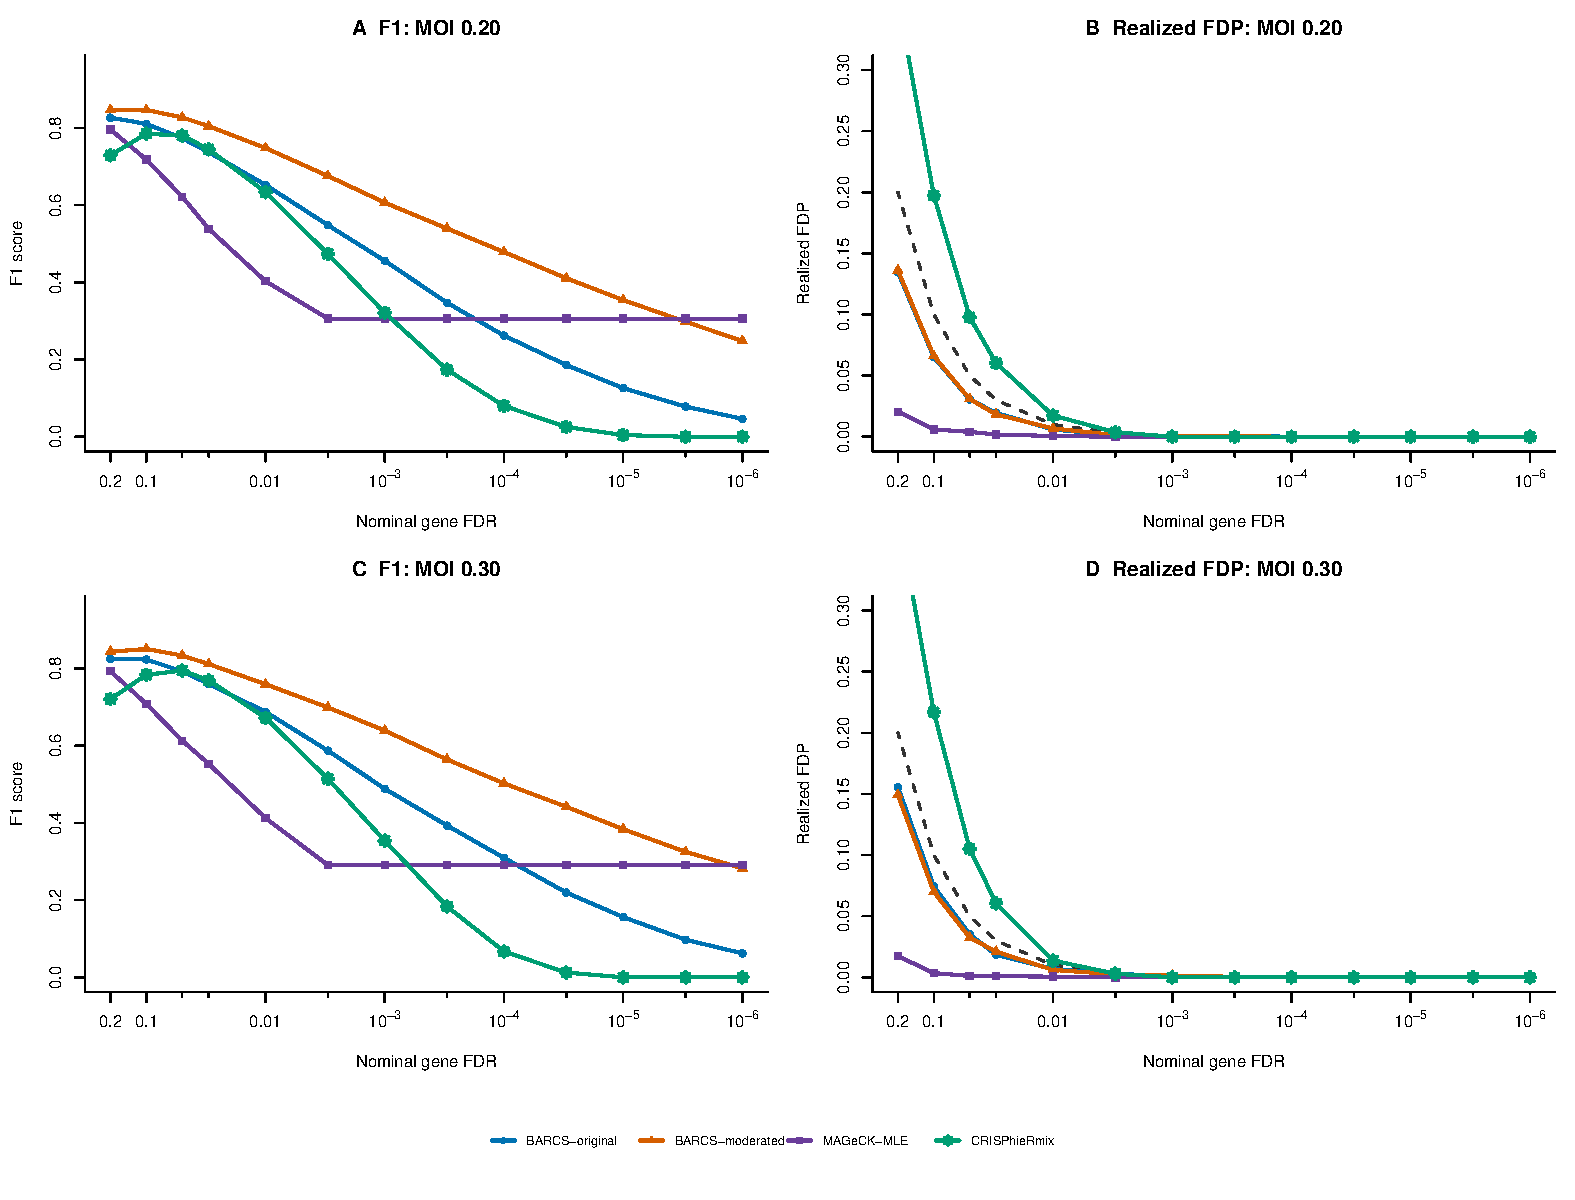
\includegraphics[width=\textwidth]{figures/crispulator_facs_moi_10k_f1_by_fdr.pdf}
\caption{Calibration and F1 across gene-FDR cutoffs in the genome-scale
simulation, means over three seeds on the common gene set.
(A) F1 and (B) realized FDP at MOI 0.20; (C) and (D) the same at MOI 0.30.
The dashed line in the FDP panels is realized equal to nominal, so a method
tracking it reports the error rate it delivers.  Thresholds above 0.10 are a
diagnostic: they show what each method could attain if its threshold were
chosen with knowledge of the truth, which a real screen does not have.}
\label{fig:crispulator-moi10k-fdr}
\end{figure}

At MOI 0.30 every one of these conclusions is reproduced.  BARCS-MOD again leads F1 at
FDP 0.070, CRISPhieRmix again attains its recall at FDP 0.217, and MAGeCK-MLE
again ranks marginally best while calling least, at FDP 0.003 and F1 0.708.
The one difference is that MAGeCK-MLE's average-precision margin over
BARCS-MOD is resolvable at this MOI, 0.0033 (0.0017 to 0.0049).  At the higher
multiplicity CRISPhieRmix marginally exceeds BARCS-MOD on directional recall,
0.785 against 0.784, but at three times the realized error rate, so the
ordering that matters is unchanged.


\paragraph{Supporting 400-gene sensitivity to MOI, guide quality, library
size, and replication.}
The remaining simulation analyses in this subsection are the earlier
400-gene grid, retained because they map the parameter boundaries that the
genome-scale benchmark deliberately does not vary, including the
one-replicate boundary.  They predate the moderated statistic and use the
historical BARCS-ST default and the earlier
$\mathrm{MOI}\in\{0.10,0.25,0.40\}$ levels, so they should be read as
boundary mapping rather than as the headline comparison.  We
varied MOI, the high-quality-guide fraction, the number of genes, and the
number of independent screen replicates one at a time, using five paired seeds
at every setting (ten unique settings and 50 simulations in total).  Nine
settings had at least three replicates; the one-replicate setting was a
prespecified diagnostic boundary.  Among the supported settings, in the
primary low--bulk--high comparison,
BARCS-minus-MAGeCK-MLE average precision ranged only from $-0.015$ to $0.022$
and changed sign across settings.  Thus this experiment does not support a
general ranking advantage for BARCS.  Its more consistent strength was
directional recovery at the prespecified FDR threshold: the directional-recall
difference was positive in seven of nine settings and ranged from $-0.018$ to
$0.136$, while the F1 difference ranged from $-0.022$ to $0.080$.

The largest directional-recall differences occurred at MOI 0.10
($+0.107$) and a high-quality-guide fraction of 0.75 ($+0.119$).  At MOI
0.40, however, MAGeCK-MLE led directional recall by $0.018$ and F1 by
$0.022$; with only 60\% high-quality guides, the methods were nearly tied on
directional recall and MAGeCK-MLE led F1 by $0.005$.  Across 100, 400, and
1,000 genes, BARCS directional-recall differences were $+0.081$, $+0.047$,
and $+0.064$, respectively, whereas average-precision differences again
remained small.  The 100-gene setting also produced realized FDP above 0.10
for both methods (0.181 for BARCS and 0.147 for MAGeCK-MLE), warning that five
small-library replicates do not establish finite-sample FDR control.  These
results sharpen the claim: BARCS can improve directionally correct thresholded
recovery under some noisy or low-MOI conditions, but neither method dominates
every metric or simulation regime.

Replication changed that comparison.  With three replicates, BARCS exceeded
MAGeCK-MLE in directional recall by 0.136 and F1 by 0.080; with four
replicates the differences were 0.047 and 0.011.  At six replicates the signs
reversed slightly, to $-0.012$ for directional recall and $-0.014$ for F1.
The practical interpretation is not that fewer replicates are desirable:
average precision, recall, and F1 increased for both methods as replication
increased.  Rather, BARCS's relative sensitivity is largest in the
low-replication regime, whereas MAGeCK-MLE becomes comparable when information is
abundant.

One replicate crossed from low information into non-confirmatory inference.
Ordinary BARCS retained higher average precision than MAGeCK-MLE, 0.633 versus
0.548, but made no discoveries at gene FDR 0.10 across the five seeds;
MAGeCK-MLE's mean directional recall was only 0.014.  The new BARCS-GC
guide-consistency statistic increased average precision to 0.670,
directional recall to 0.145, and F1 to 0.245.  It made 58 calls across the
five simulations (3--19 per seed), all of which were active genes under the
simulated truth, for mean realized FDP 0.  The fitted empirical-null scales
were 2.19--2.60, showing why an unscaled Wald reference would have been
anti-conservative.

This improvement is useful but deliberately narrow.  BARCS-GC asks whether
independently designed guides give concordant signed effects and assumes that
fewer than half of genes are active; it does not create biological replication.
Its empirical-null calls are therefore hypothesis-generating, not
confirmatory.  We recommend an independent screen for confirmation even when
BARCS-GC is used to prioritize genes from an otherwise irreplaceable $R=1$
experiment.



\noindent\begin{minipage}{\textwidth}
At the four-replicate baseline, mean core fitting times were 0.35 seconds for
BARCS and 4.34 seconds for MAGeCK-MLE.  These measurements exclude
simulation, file input/output, and guide-to-gene aggregation; they show that
the broader comparison is computationally practical but should not be read as
an end-to-end software benchmark.
\end{minipage}

\clearpage

% !TeX root = ../../main.tex
\subsection{Control denominators recover interactions under composition shifts}
\label{sec:simcrispr}

We next used simCRISPR to generate a factorial knockout-by-treatment screen
with a known guide-level interaction \citep{zhu2026simcrispr}.  Each of three
seeds contained 2,000 sgRNAs and three independent replicates per factorial
arm.  Non-targeting guides had a true interaction of zero, and safe-harbor
guides separated the effect of cutting from a targeted gene effect.  Each
control class was split so that normalization and calibration guides were
never used for evaluation.

\begin{table}[ht]
\centering
\caption{Interaction recovery in simCRISPR (three-seed mean).  Recall and F1
use targeting guides with $|\mathrm{interaction}|\geq0.2$ as positives.  Null
and safe-harbor rates are held-out call fractions at FDR 0.10.}
\label{tab:simcrispr}
\small
\setlength{\tabcolsep}{5pt}
\begin{tabular}{llrrrr}
\toprule
Method & Denominator & Dir.\ recall & F1 & Null rate & Safe-harbor\\
\midrule
BARCS-ST & Library &
0.376 & 0.488 & 0.004 & 0.002\\
BARCS-MOD & Library &
0.375 & 0.481 & 0.000 & 0.000\\
\midrule
BARCS-ST & Non-targeting &
0.769 & 0.870 & 0.024 & 0.070\\
BARCS-MOD & Non-targeting &
\textbf{0.838} & \textbf{0.917} & 0.040 & 0.080\\
\midrule
BARCS-ST & Safe-harbor &
0.762 & 0.864 & 0.042 & 0.042\\
BARCS-MOD & Safe-harbor &
0.830 & 0.914 & 0.027 &
\textbf{0.035}\\
\midrule
MAGeCK-MLE & Non-targeting &
0.003 & 0.006 & 0.000 & 0.000\\
\bottomrule
\end{tabular}
\end{table}

The full-library denominator preserved effect ranking but shifted the
true-zero guides because widespread depletion increased every surviving
guide's library share.  BARCS-MOD consequently reached F1 0.481 with the
library denominator, compared with 0.917 and 0.914 using non-targeting and
safe-harbor denominators.  The held-out null rates remained below the nominal
0.10 in all cases.  The result identifies denominator choice, rather than the
interaction coefficient itself, as the source of the power loss.

\begin{figure}[htbp]
\centering
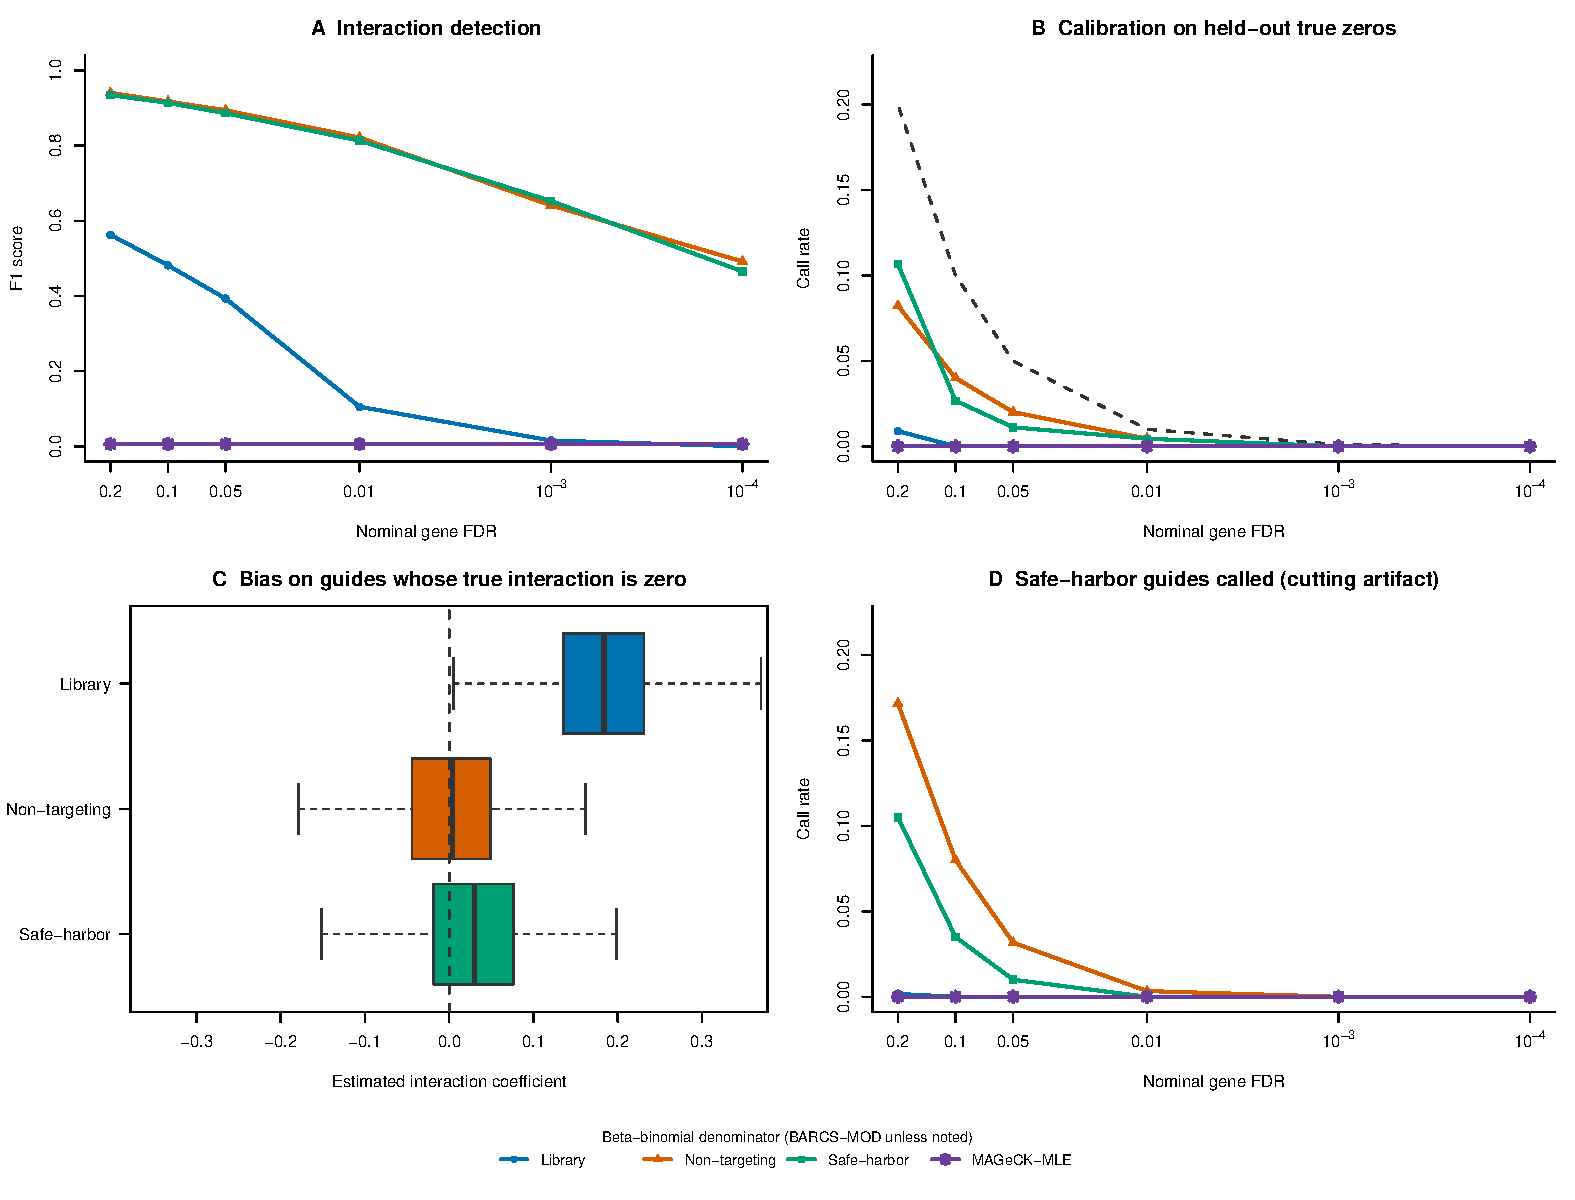
\includegraphics[width=\textwidth]{figures/simcrispr_interaction.pdf}
\caption{\textbf{Denominator choice controls interaction recovery.}  (A)
Estimated interactions among true-zero guides.  A full-library denominator
induces a positive shift; either control denominator removes it.  (B) F1
across requested FDR thresholds.  Control denominators retain substantially
more interaction power.}
\label{fig:simcrispr}
\end{figure}

The two control denominators performed similarly overall but differed on
cutting artifacts.  Safe-harbor guides were called at 0.080 after
non-targeting normalization and 0.035 after safe-harbor normalization.
Non-targeting controls are therefore efficient for detecting targeted
interactions, whereas safe-harbor controls better absorb the shared cutting
response.  MAGeCK-MLE is shown only as a reference: the simulated truth is
guide-level, leaving no within-gene replication for its native gene model.

% !TeX root = ../../main.tex
\subsection{A multi-coefficient design on real data: GSE70038}

The benchmarks so far test one coefficient at a time.  GSE70038 is the case
where the design matrix earns its place: 64,747 guides in 16 libraries from two
glioblastoma stem-cell lines and two neural stem-cell lines, with duplicate
initial and terminal samples \citep{toledo2015pkmyt1}.  The scientific target is
four cell-line-specific terminal effects estimated \emph{jointly} against one
shared initial baseline.  Four separate two-group tests cannot express that: each
would re-estimate the baseline from its own pair, discarding the other twelve
libraries that inform it.  This is therefore not a continuous-phenotype
benchmark but the multivariable one, and it is the design MAGeCKFlute documents
as the canonical multi-condition layout.

We followed the design-matrix rules in Table~5 and Box~3 of the MAGeCKFlute
protocol \citep{wang2019mageckflute}.  The first column is one for every
library; each initial library has zeros elsewhere; and each terminal library
has one in exactly one of four cell-line columns.  The same $16\times5$ matrix
was supplied to beta-binomial regression and the official MAGeCK-MLE 0.5.9.5
executable.  MAGeCK used median normalization and its Wald inference.  For the
beta-binomial result, guide effects were summarized by their within-gene
median, and directional guide $p$-values were combined by Stouffer's method.
This aggregation is an explicit comparison device, not a proposed replacement
for MAGeCK's gene model.

The ``effect rank correlation'' reported below is calculated in this analysis,
not copied from GEO or the MAGeCKFlute paper.  Separately for each terminal
coefficient, we pair all genes available from both methods.  The
beta-binomial effect is the within-gene median guide coefficient, and the
MAGeCK effect is its official MLE beta.  We assign average ranks to these two
effect vectors and take their Pearson correlation, which is exactly Spearman's
rank correlation.  The 18,077 paired effects and their ranks for every
coefficient are included with the deposited analysis output.

\begin{table}[ht]
\centering
\caption{Effect concordance between \methodswatch{barcsblue} BARCS and
\methodswatch{mageckorange} official MAGeCK-MLE on GSE70038.  Jaccard is the
overlap divided by the union of the 200 most depleted genes from each method.
Higher agreement is better; column maxima are shown in bold.}
\label{tab:gse}
\begin{tabular}{lrr}
\toprule
Terminal coefficient & Spearman effect correlation & Top-200 Jaccard\\
\midrule
GSC0131 & \textbf{0.928} & 0.550\\
GSC0827 & 0.888 & 0.533\\
NSCCB660 & 0.905 & 0.544\\
NSCU5 & 0.915 & \textbf{0.562}\\
\bottomrule
\end{tabular}
\end{table}

Concordance here is the validation rather than the finding.  The comparison is
not circular: beta-binomial regression conditions on each library total, whereas
MAGeCK uses a normalized negative-binomial count model with guide-efficiency
estimation \citep{li2015mageckvispr}.  Two models that disagree on the noise
distribution, the normalization, and the guide-efficiency treatment nevertheless
place the four coefficient vectors in the same order, with all four effect
correlations above 0.88.  That is the evidence that the model-matrix interface
recovers the intended estimand on a real screen rather than a reparameterised
approximation of it.  These correlations
measure agreement of the inferred gene ordering; they are not likelihood,
calibration, or predictive-fit statistics and therefore cannot identify a
better-fitting method.  In GSC0131, the
published convergent dependency PKMYT1 has effect $-0.987$ and FDR
$1.87\times10^{-8}$ under beta-binomial regression, versus beta $-0.786$ and
Wald FDR $4.53\times10^{-8}$ under MAGeCK-MLE.  Both also recover HEATR1,
TFAP2C, and WEE1 depletion.  Figure~\ref{fig:gse} shows the complete GSC0131
comparison; the reproducible PDF contains one page per terminal coefficient.

\begin{figure}[ht]
\centering
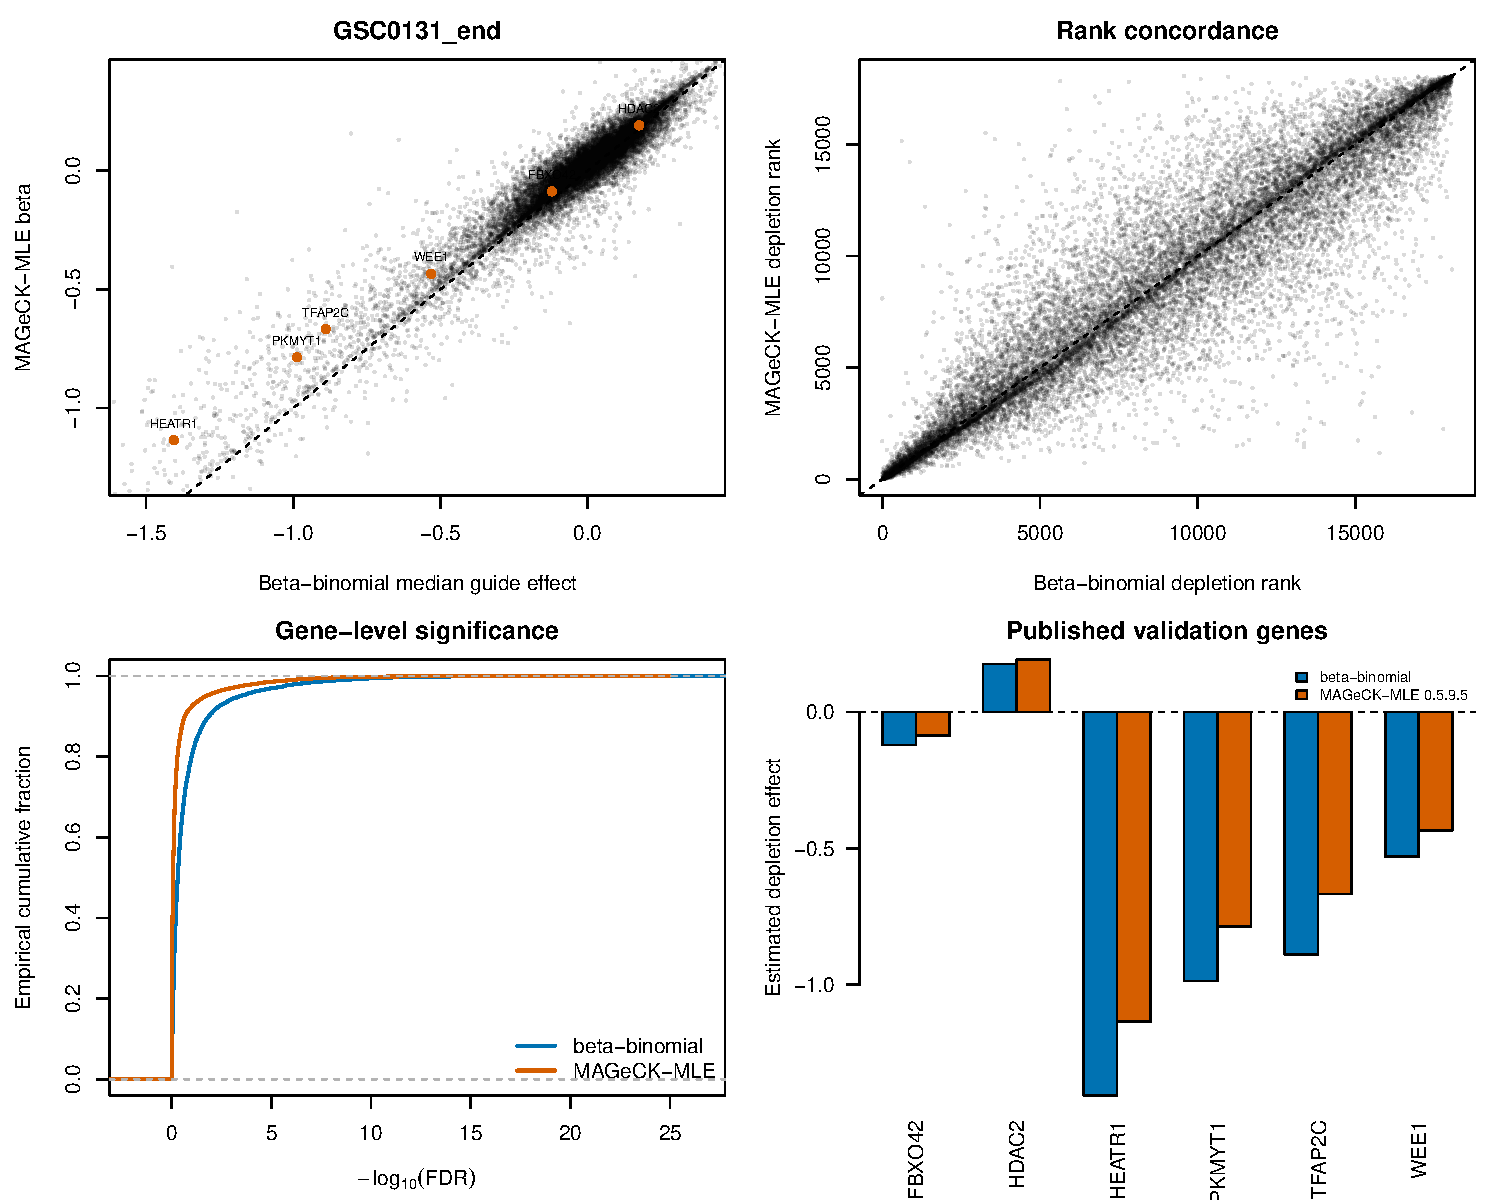
\includegraphics[width=\textwidth]{figures/gse70038_head_to_head.pdf}
\caption{GSE70038 GSC0131 head-to-head.  (A) Gene effects, with dark points
marking the prespecified genes PKMYT1, HEATR1, TFAP2C, FBXO42, HDAC2, and WEE1.
(B) Depletion-rank concordance.  (C) Gene-level FDR distributions.  (D)
Effects for the published validation genes.}
\label{fig:gse}
\end{figure}
\clearpage

% !TeX root = ../../main.tex
\subsection{Endpoint benchmark and copy-number audit}

To ask which method ranks biological dependencies better, we used the
Brunello A375 negative-selection screen of \citet{sanson2018optimized}, bundled
with CB\textsuperscript{2}.  This is an ordinary endpoint screen rather than a
continuous-phenotype experiment, but it supplies an external target unavailable
in GSE70038: reference essential genes should rank ahead of reference
nonessential genes \citep{hart2017evaluation}.  The beta-binomial score combines guide
evidence by directional Stouffer aggregation; the MAGeCK score uses the
official MLE beta and Wald $p$-value.  Both are oriented so larger scores mean
stronger depletion.

\subsubsection{Copy-number-aware analysis}

Copy number is a gene-level property of A375, not a sample-level covariate:
for a given guide it is constant across the plasmid and three terminal
libraries.  Adding it directly to the four-row sample design would therefore
be non-identifiable with the endpoint effect.  Instead, we downloaded the
A375 gene-level profile (ACH-000219) from DepMap Public 19Q3
\citep{depmap19q3,meyers2017cnv} and used MAGeCK 0.5.9.5's official
\texttt{--cnv-norm} piecewise correction.  For an apples-to-apples comparison,
the same MAGeCK piecewise normalizer was applied to the beta-binomial
within-gene median effects.  It adjusts effect sizes after model fitting; it
does not refit either count likelihood.  The common CNV-complete evaluation set
contains 1,506 essential and 869 nonessential genes.

\begin{table}[ht]
\centering
\caption{CNV-aware Sanson A375 benchmark.  The final column is Spearman
correlation between effect and copy number among reference nonessential genes;
values nearer zero indicate less residual CNV-associated depletion.  F1 uses
nominal FDR 0.05 and a negative effect.  Higher discrimination metrics and
CNV correlation closest to zero are highlighted.}
\label{tab:sanson}
\small
\setlength{\tabcolsep}{4pt}
\begin{tabular}{lrrrr}
\toprule
Method & AUROC & Avg. precision & F1 & CNV correlation\\
\midrule
\methodswatch{barcsblue} BARCS &
  \textcolor{barcsblue}{\textbf{0.9598}} & 0.9786 &
  \textcolor{barcsblue}{\textbf{0.8531}} & $-0.185$\\
\methodswatch{barcsblue} BARCS + CNV &
  0.9533 & 0.9762 & \textcolor{barcsblue}{\textbf{0.8531}} & $-0.042$\\
\methodswatch{mageckorange} Official MAGeCK-MLE &
  \textcolor{mageckorange}{\textbf{0.9598}} &
  \textcolor{mageckorange}{\textbf{0.9795}} &
  0.8277 & $-0.207$\\
\methodswatch{mageckorange} Official MAGeCK-MLE + CNV &
  0.9501 & 0.9762 & 0.8277 &
  \textcolor{mageckorange}{$\mathbf{-0.006}$}\\
\bottomrule
\end{tabular}
\end{table}

CNV correction substantially removes the intended nuisance association:
$-0.185$ to $-0.042$ for beta-binomial effects and $-0.207$ to $-0.006$ for
MAGeCK.  It does not improve essential-gene discrimination in this screen.
AUROC decreases by 0.0066 and 0.0097, respectively, and the 0.05-FDR calls are
unchanged.  This is not a contradiction: bias removal and gold-standard
classification are different targets, and amplified genes can include both
dependencies and nondependencies.

After CNV correction, beta-binomial versus MAGeCK global ranking remains
indistinguishable: the AUROC difference is 0.00316 (paired
stratified-bootstrap 95\% CI $-0.00265$ to $0.00924$), and the average
precision difference is effectively zero (95\% CI $-0.00349$ to $0.00295$).
At nominal FDR 0.05, beta-binomial retains 4.18 percentage points more recall
(95\% CI 2.66 to 5.71) and an F1 advantage of 0.0253 (95\% CI 0.0148 to
0.0362).

% !TeX root = ../../main.tex
\subsection{False-discovery conclusions depend on the analysis contract}
\label{sec:fdr-audit}

We audited a deposited Chronos benchmark that compared CB\textsuperscript{2},
MAGeCK, JACKS, DrugZ, and Chronos \citep{dempster2025fdr,
dempster2025fdrdata}.  The key issue was the beta-binomial denominator.  In
the reported null-only Avana analysis, the count matrix was restricted to
control genes before fitting, so its column sums no longer represented full
sequencing depth.  Reusing the full-library CB\textsuperscript{2} probabilities
for the same test genes changed the number of FDR 0.10 discoveries from 152 to
zero.

\begin{table}[htbp]
\centering
\caption{Data-driven audit of the external false-discovery benchmark.
``Known'' refers to the 28 literature-curated condition--gene combinations,
not a complete truth set.}
\label{tab:chronosaudit}
\small
\setlength{\tabcolsep}{4pt}
\begin{tabular}{p{0.18\textwidth}p{0.17\textwidth}p{0.15\textwidth}
                p{0.16\textwidth}p{0.20\textwidth}}
\toprule
Audit & Reference set & Reported result & Full-total reanalysis &
Additional diagnostic\\
\midrule
Avana null-only &
Null genes, five cell lines &
152 calls at FDR 0.10 &
0 calls at FDR 0.10 &
Largest null $p<0.05$ rate: 0.145\\
PSN1 two-versus-two split &
Null pseudo-condition &
0 gene calls &
0 gene calls &
Guide $p<0.05$: 0.0481 raw, 0.0465 scaled\\
DeWeirdt differential screens &
28 curated interactions &
0/28 known recovered &
38 calls; 1/28 known recovered &
37/38 calls arose in one comparison\\
\bottomrule
\end{tabular}
\end{table}

The PSN1 result shows that pooling one guide dispersion across the design can
avoid the extreme loss of power produced by separate two-replicate variance
estimates while retaining a near-nominal guide null.  The DeWeirdt result shows
the boundary of that improvement: BARCS recovered only MCL1 under A-1331852,
and nearly all other calls came from one OVCAR8--olaparib comparison without
recovering BRCA1 or BRCA2.  A global treatment-associated quality shift cannot
be separated from treatment with only two replicates per arm.

These results do not establish a winner against a complete ground truth.
They show that pre-fit guide subsetting and common normalization can alter the
effective depth seen by a library-total-conditional model.  Comparator studies
must preserve full-library totals, separate calibration guides from evaluation
guides, and use blocked permutations or independent validation for
differential screens.



\section{Methods}
% !TeX root = ../main.tex
% Methods subsections, in narrative order.
% !TeX root = ../../main.tex
\subsection{\texorpdfstring{From CB\textsuperscript{2} to
BARCS}{From CB2 to BARCS}}

BARCS is fundamentally a guide-level coefficient model.  Its required inputs
are a guide-by-library count matrix, the corresponding full-library totals,
and a sample design matrix; its primary output is one coefficient or contrast
test per guide.  Gene aggregation is downstream and optional.  In particular,
neither Fisher nor Stouffer combination is required to fit or interpret the
BARCS regression.  Some benchmarks below use an explicitly labeled Stouffer
summary to compare with deposited gene-level results, whereas BARCS-GC uses
the direct shared-effect Wald construction in
Equations~\eqref{eq:guideconsistency}--\eqref{eq:gcz}.

CB\textsuperscript{2} adapts the beta-binomial weighted test of
\citet{baggerly2003differential} to CRISPR pooled screens
\citep{jeong2019beta}.  Its central insight is worth preserving: sequencing
depth measures a guide proportion precisely, but it does not turn reads into
independent biological replicates.  The original method applies this insight
to a two-group contrast.  BARCS retains the same
depth-aware, extra-binomial variance principle and changes the mean model from
two group means to a design matrix.  ``Retains'' refers to the stochastic
hierarchy and the sample-level information ceiling; it does not mean that the
default logit fit reproduces the original finite-sample statistic.  The
legacy representation and asymptotic relationship are established below.

\begin{table}[ht]
\centering
\caption{What changes---and what does not---from the original
CB\textsuperscript{2} method to BARCS.}
\label{tab:cb2difference}
\small
\setlength{\tabcolsep}{5pt}
\begin{tabular}{p{0.20\textwidth}p{0.32\textwidth}p{0.38\textwidth}}
\toprule
Feature & \methodswatch{cbtwocyan} Original CB\textsuperscript{2} &
\methodswatch{barcsblue} BARCS\\
\midrule
Primary question & Difference between two groups &
Trend, adjusted association, interaction, or contrast\\
Sample design & Reference and comparison labels &
Arbitrary full-rank R model matrix\\
Mean model & Two unrelated group proportions &
$\logit(\mu_i)=\mathbf{x}_i^\top\boldsymbol{\beta}$\\
Effect & Difference or fold change between groups &
Conditional log-odds coefficient or linear contrast\\
Dispersion & Separate beta-binomial weighting within each group &
One guide-specific $\rho$ shared across the fitted design\\
Estimator & Weighted group proportions &
Feasible logistic IRLS\\
Variance principle & \multicolumn{2}{c}{Binomial sequencing plus
between-library beta-binomial heterogeneity}\\
Reference df & Group-variance df formula &
Residual $m-q$\\
Adjustment & Pairwise stratification or preprocessing &
Batch, donor, dose, time, interactions, splines, and other covariates\\
Implementation & Existing CB\textsuperscript{2} workflow &
Additive \texttt{bbreg()}, \texttt{bb\_contrast()}, and
\texttt{bb\_screen()} APIs with RcppArmadillo kernels\\
\bottomrule
\end{tabular}
\end{table}

The regression bridge was described by \citet{baggerly2004overdispersed} for
sequencing count data with multiple groups and continuous covariates.  The
method combines logistic regression with extra-binomial variation and retains
a coefficient-based $t$ test.  Here we state that construction in CRISPR-screen
notation and use the beta-binomial, library-size-dependent variance of
\citet{williams1982extrabinomial}.  An identity-link regression of raw
proportions would allow fitted values outside $(0,1)$, while an unweighted
correlation would ignore unequal library sizes.  The logit and beta-binomial
weights solve those two problems directly.

% !TeX root = ../../main.tex
\subsection{Model}

For guide $g$ in sequenced sample $i$, let $K_{gi}$ be its read count, let
$N_i$ be the full mapped-guide total for that sample, and let
$Y_{gi}=K_{gi}/N_i$ be the observed guide proportion.  Sample-level
quantities such as dose, time, treatment, donor, and batch are predictors even
when they are described biologically as experimental ``outcomes.''

The model is fitted separately for every guide, so the guide index is
suppressed below.  Conditional on a latent sample-specific abundance $P_i$,
\begin{align}
  K_i \mid P_i &\sim \operatorname{Binomial}(N_i,P_i),\\
  P_i &\sim \operatorname{Beta}(\mu_i\kappa,(1-\mu_i)\kappa).
\end{align}
The mean is linked to a row vector of sample covariates $\mathbf{x}_i^\top$ by
\begin{equation}
  \logit(\mu_i)
  = \log\left(\frac{\mu_i}{1-\mu_i}\right)
  = \mathbf{x}_i^\top\boldsymbol{\beta}.
  \label{eq:mean}
\end{equation}
The design can contain an intercept, a continuous phenotype, batch indicators,
interactions, spline terms, and other prespecified adjustment variables.

It is useful to express the beta precision $\kappa$ as an intraclass
correlation
\begin{equation}
  \rho = \frac{1}{\kappa+1}, \qquad 0\leq\rho<1.
\end{equation}
Marginally,
\begin{align}
  \E(K_i) &= N_i\mu_i,\\
  \Var(K_i) &=
  N_i\mu_i(1-\mu_i)\{1+(N_i-1)\rho\}, \label{eq:countvar}\\
  \Var(Y_i) &=
  \mu_i(1-\mu_i)
  \left\{\frac{1-\rho}{N_i}+\rho\right\}. \label{eq:propvar}
\end{align}
Equation~\eqref{eq:propvar} cleanly separates sequencing uncertainty, which
decreases with $N_i$, from between-sample heterogeneity, which does not vanish
when sequencing depth becomes arbitrarily large.

\subsubsection{Interpretation of the continuous coefficient}

Suppose the model contains a continuous phenotype $d_i$ with coefficient
$\beta_d$.  Then $\exp(\beta_d)$ is the multiplicative change in the odds of
observing that guide for a one-unit increase in $d_i$, conditional on the other
covariates.  Standardizing $d_i$ before fitting makes $\exp(\beta_d)$ the odds
ratio per sample standard deviation and makes guide effects directly
comparable.  For rare guides, odds and proportions are similar, so $\beta_d$ is
also approximately a log abundance ratio per unit of $d_i$.

\input{sections/methods/2_estimation-irls}
% !TeX root = ../../main.tex
\subsection{T-based inference}

At convergence, the model-based covariance estimator is
\begin{equation}
  \widehat{\operatorname{Cov}}
  (\widehat{\boldsymbol{\beta}})
  =(X^\top\widehat{W}X)^{-1}.
  \label{eq:covariance}
\end{equation}
The Pearson equation scales the residual variation to approximately one.  If
the dispersion estimate reaches its numerical upper boundary, the
implementation additionally multiplies Equation~\eqref{eq:covariance} by the
remaining Pearson scale.

Equation~\eqref{eq:covariance} is a plug-in, model-based covariance: it
conditions on the estimated $\widehat{\rho}$ as though it were fixed.  It does
not propagate uncertainty from estimating a separate dispersion for every
guide.  Referring the coefficient to $t_{m-q}$ gives a heavier-tailed
small-sample reference than a normal approximation, but it is not a formal
correction for dispersion-estimation uncertainty.  With few independent
libraries, calibration must therefore be checked by simulation, phenotype
permutation, or prespecified negative controls.

For coefficient $\beta_j$, the statistic
\begin{equation}
  t_j =
  \frac{\widehat{\beta}_j-\beta_{j,0}}
  {\sqrt{
  \widehat{\operatorname{Cov}}
  (\widehat{\boldsymbol{\beta}})_{jj}}}
  \label{eq:tstat}
\end{equation}
is compared with a Student $t_{m-q}$ distribution.  The degrees of freedom are
driven by the number of independent sequenced samples, not by the total read
count.  This is the crucial reason that a library with millions of reads does
not create artificial certainty.

More generally, for a prespecified contrast vector $\mathbf{c}$,
\begin{equation}
  t_{\mathbf{c}} =
  \frac{\mathbf{c}^\top\widehat{\boldsymbol{\beta}}-\delta_0}
  {\sqrt{\mathbf{c}^\top
  \widehat{\operatorname{Cov}}(\widehat{\boldsymbol{\beta}})
  \mathbf{c}}}
\end{equation}
uses the same $m-q$ degrees of freedom.  This covers pairwise group contrasts,
average slopes in interaction models, and other one-degree-of-freedom
hypotheses.  Guide-wise two-sided $p$-values are adjusted using the
Benjamini--Hochberg procedure \citep{benjamini1995controlling}.

\subsubsection{From guide statistics to gene statistics}

BARCS fits the count model guide by guide.  The primary HT-29, FACS,
simulation, GSE70038, and A375 benchmark scripts then use an explicit
directional Stouffer summary, denoted BARCS-ST below, to obtain one gene-level
statistic.
For the $j$th valid guide targeting gene $g$, the two-sided guide $p$-value is
converted back to a signed standard-normal score,
\begin{equation}
  z_{gj}
  =
  \operatorname{sign}(\widehat{\beta}_{gj})
  \Phi^{-1}\!\left(1-\frac{p_{gj}}{2}\right).
  \label{eq:signedz}
\end{equation}
If $m_g$ valid guides target the gene, their combined score and two-sided
gene-level $p$-value are
\begin{equation}
  Z_g=\frac{1}{\sqrt{m_g}}\sum_{j=1}^{m_g}z_{gj},
  \qquad
  p_g=2\Phi(-|Z_g|).
  \label{eq:genestouffer}
\end{equation}
The reported gene effect is the median of the guide coefficient estimates,
\begin{equation}
  \widehat{\beta}_g
  =\operatorname{median}_{j=1,\ldots,m_g}
    \widehat{\beta}_{gj},
  \label{eq:geneeffect}
\end{equation}
and gene-level false-discovery rates are obtained by applying
Benjamini--Hochberg to the collection of $p_g$ values.  Consequently,
concordant guide directions reinforce one another, discordant directions
cancel, and one extreme guide has limited influence on the reported effect.

This aggregation is deliberately transparent, but it is not a native
hierarchical gene model.  Equations~\eqref{eq:signedz}--\eqref{eq:genestouffer}
give equal weight to valid guides and use the independence reference
$\sqrt{m_g}$; shared sequence artifacts or other correlation can therefore
make the gene statistic anti-conservative.  A production extension should
estimate guide reliability and within-gene dependence or use a hierarchical
effect model.  In the biological head-to-head benchmarks, this
Stouffer--median procedure is used only for BARCS (and for the deliberately
naive binomial comparator).  MAGeCK, Chronos, BAGEL2, Waterbear, and MAUDE
retain their native or deposited gene-level summaries.  The exploratory
DeWeirdt false-discovery audit used Fisher aggregation as stated in its
Results description and is not pooled with these primary benchmark
statistics.

\paragraph{Exchangeable normal guide-beta statistic.}
BARCS-NORM implements a different and deliberately simple model.  It does not
transform guide $p$-values and does not use guide-specific standard errors.
Instead, for the $m_g$ valid guides targeting gene $g$, it assumes
\begin{equation}
  \widehat{\beta}_{gj}
  \mathrel{\overset{\mathrm{iid}}{\sim}}
  N(\mu_g,\sigma_g^2).
  \label{eq:genenormal}
\end{equation}
The gene effect and between-guide standard deviation are estimated directly:
\begin{align}
  \widehat{\mu}_g
  &=
  \frac{1}{m_g}\sum_{j=1}^{m_g}\widehat{\beta}_{gj},\\
  s_g^2
  &=
  \frac{1}{m_g-1}
  \sum_{j=1}^{m_g}
  (\widehat{\beta}_{gj}-\widehat{\mu}_g)^2.
\end{align}
Testing $H_0:\mu_g=0$ gives
\begin{equation}
  T_g
  =
  \frac{\widehat{\mu}_g}{s_g/\sqrt{m_g}}
  \sim t_{m_g-1}
  \quad\text{under Equation~\eqref{eq:genenormal} and }H_0.
  \label{eq:genenormalt}
\end{equation}
Thus normally distributed guide betas lead to a Student $t$ reference when
their unknown $\sigma_g$ is estimated from the same guides.  The software also
reports $2\Phi(-|T_g|)$ as a plug-in normal sensitivity value, but it is not
the primary $p$-value because it treats the estimated spread as known.
Multiple guides support this guide-consistency calculation; they do not become
additional biological screen replicates.

\paragraph{Random-effects and moderated random-effects statistics.}
BARCS-RE (the implementation label \texttt{BARCS-partial}) retains each
guide-specific regression standard error and models
\begin{equation}
  \widehat{\beta}_{gj}\mid\beta_g,\tau_g^2
  \sim
  N\!\left(
    \beta_g,\,
    \operatorname{SE}(\widehat{\beta}_{gj})^2+\tau_g^2
  \right).
  \label{eq:generandomeffects}
\end{equation}
It estimates $\tau_g^2$ by the nonnegative DerSimonian--Laird estimator
\citep{dersimonian1986meta} and then pools guide effects with weights
\begin{equation}
  w_{gj}
  =
  \left\{
    \operatorname{SE}(\widehat{\beta}_{gj})^2+
    \widehat{\tau}_g^2
  \right\}^{-1},
  \qquad
  \widehat{\beta}_g
  =
  \frac{\sum_jw_{gj}\widehat{\beta}_{gj}}{\sum_jw_{gj}}.
  \label{eq:genere}
\end{equation}
BARCS-RE-EB (implementation label \texttt{BARCS-EB}) stabilizes the noisy
gene-specific heterogeneity estimate by shrinking it toward the pooled
screen-wide excess-$Q$ estimate $\tau_0^2$:
\begin{equation}
  \widetilde{\tau}_g^2
  =
  \frac{
    (m_g-1)\widehat{\tau}_g^2+d_0\tau_0^2
  }{
    (m_g-1)+d_0
  },
  \qquad d_0=4.
  \label{eq:geneeb}
\end{equation}
Both random-effects statistics are calibrated against prespecified
negative-control genes when at least ten are available and otherwise against a
robust whole-screen empirical null.  In contrast, BARCS-NORM obtains its
spread and reference degrees of freedom entirely within each gene.  These
three alternatives and BARCS-ST reuse exactly the same fitted guide
coefficients; only the guide-to-gene inference changes.

\paragraph{Guide-consistency statistic for the one-replicate boundary.}
When sample replication is insufficient, converting a guide statistic through
a low-degree-of-freedom $t$ distribution can erase useful ranking information.
We therefore prespecified a separate exploratory gene statistic, BARCS-GC,
for the $R=1$ CRISPulator analysis.  It uses the uncalibrated guide
coefficient and model-based standard error to estimate one shared gene effect.
With
\begin{equation}
  w_{gj}
  =
  \operatorname{SE}(\widehat{\beta}_{gj})^{-2},
\end{equation}
the inverse-variance estimate, its standard error, and raw Wald statistic are
\begin{equation}
  \widehat{\beta}_g
  =
  \frac{\sum_{j=1}^{m_g}w_{gj}\widehat{\beta}_{gj}}
       {\sum_{j=1}^{m_g}w_{gj}},
  \qquad
  \operatorname{SE}(\widehat{\beta}_g)
  =
  \left(\sum_{j=1}^{m_g}w_{gj}\right)^{-1/2},
  \qquad
  T_g
  =
  \frac{\widehat{\beta}_g}
       {\operatorname{SE}(\widehat{\beta}_g)}.
  \label{eq:guideconsistency}
\end{equation}
This is a direct fixed-effect estimate of the common guide coefficient, not a
Fisher or Stouffer combination of guide $p$-values.  Its additional assumption
is that the guide coefficients target one common gene effect; the reported
direction-agreement fraction exposes gross heterogeneity.

Because $T_g$ does not have a trustworthy sample-replicate reference
distribution at $R=1$, it is calibrated across genes.  Let $c_0$ be the
all-gene median and
\begin{equation}
  s_{\mathrm{MAD}}
  =
  \frac{\operatorname{median}_g|T_g-c_0|}
       {\Phi^{-1}(0.75)}.
  \label{eq:gcmad}
\end{equation}
When at least ten valid control genes are present, let $c_C$ be their median
and let
\begin{equation}
  s_C
  =
  \frac{Q_{0.95}\{|T_g-c_C|:g\in C\}}
       {\Phi^{-1}(0.975)}.
  \label{eq:gccontrol}
\end{equation}
The calibrated statistic and two-sided empirical-null $p$-value are
\begin{equation}
  Z_g^{\mathrm{GC}}
  =
  \frac{T_g-c_C}{\max(1,s_{\mathrm{MAD}},s_C)},
  \qquad
  p_g^{\mathrm{GC}}
  =
  2\Phi(-|Z_g^{\mathrm{GC}}|),
  \label{eq:gcz}
\end{equation}
followed by Benjamini--Hochberg adjustment.  If too few control genes are
available, $c_0$ replaces $c_C$ and $s_C$ is omitted.  At least three finite
guide coefficient estimates are required per gene.  The all-gene MAD assumes
that fewer than half of tested genes are active.

BARCS-GC measures reproducibility across independently designed
perturbations; it does not turn guides into independent biological samples.
Its $p$-value is consequently labeled empirical-null guide-consistency
evidence, not sample-level confirmation.  The ordinary BARCS result remains
the primary analysis when biological replicates are available, and
independent experimental replication remains necessary for confirmatory
claims.

% !TeX root = ../../main.tex
\subsubsection{Longitudinal HT-29 benchmark}

Guide counts for the HT-29 time course of \citet{tzelepis2016dropout} were
obtained from Data S2 of that article, file
\texttt{grna\_counts\_HT29C-clone3\_d7-25-HT1080.txt}, retrieved from the Europe
PMC supplementary bundle for PMC5081405.  The three sequencing columns reported
at each of days 7, 10, 13, 16, 19, 22, and 25 were summed to one column per
harvest and combined with the pDNA measurement, and guides with fewer than 30
pDNA reads were removed, leaving 86,882 guides targeting 17,995 genes.  Library
totals were computed before that filter and never recomputed, so the
beta-binomial denominator remains the full mapped-read total for each sample;
the filter removes 4.2\% of guides but only 0.10\% of reads, uniformly across
samples.  BARCS
and official MAGeCK-MLE 0.5.9.5 were both fitted to this eight-column matrix
under an identical design, in which pDNA is day 0 and the tested predictor is
day divided by 25, so the two continuous-time fits differ only in the
likelihood.  A minimum total count of 30 was applied within the BARCS fit.

Comparator effects were not recomputed.  The joint Chronos, per-endpoint
MAGeCK, and per-endpoint BAGEL2 effect matrices were taken as deposited in
Chronos Figshare article 14067047 \citep{chronosfigshare2021}, as were the
reference essential and nonessential gene lists; the corresponding individual
file identifiers are 26548532, 26548541, 30847513, 26548550, and 26548553.  As
Those two matrices carry one column per day; the day-25 column is used
directly, so the comparator is a single observed endpoint at the deepest time
point rather than a summary across days.

Two external annotations define the evaluation sets.  Positives are the
deposited reference essential genes.  Negatives are HT-29 genes with DepMap
Public 20Q2 expression below 0.5, taken from the ACH-000552 column of Figshare
file 26548487, which is the expression source used for the same threshold in the
deposited Chronos analysis.  The copy-number audit uses the ACH-000552 column of
Figshare file 26548484 \citep{depmap20q2}, and correction was performed with
MAGeCK 0.5.9.5's official piecewise \texttt{--cnv-norm} normalizer applied after
model fitting.  Because that profile was measured independently of the screen,
cell-line drift is a limitation of the copy-number analysis.

The analysis is reproduced by \repofile{examples/chronos_tzelepis_benchmark.R},
which calls the MAGeCK executable through \repofile{scripts/mageck_compat.py}
and \repofile{scripts/mageck_cnv_correct.py} and writes the tables reported
here.  Provenance for each downloaded input is recorded in
\repofile{data/raw/chronos/README.md}.

% !TeX root = ../../main.tex
\subsubsection{CRISPulator FACS benchmark}

We used CRISPulator 0.5.1's documented interfaces for library construction,
transfection, FACS selection, and sequencing \citep{nagy2017crispulator}.
The committed Julia environment pins the tagged source revision.  For each
simulation seed, one CRISPRn guide library was constructed and reused across
four independently seeded transfection, sorting, and sequencing replicates.
The default CRISPulator phenotype mixture was retained: 75\% inactive, 5\%
negative-control, 10\% phenotype-increasing, and 10\%
phenotype-decreasing genes.  The headline screens contained 10,000 genes and
five guides per gene, so 50,000 guides, which is the order of a genome-wide
library rather than a pilot.  The default guide-quality mixture---90\%
complete-knockout guides and 10\% low-activity guides---was retained.
Transfection representation was 500 cells per guide, Gaussian phenotype noise
was 2, sorting representation was 50 cells per guide, and sequencing depth was
50 reads per guide per sample.  Multiplicity of infection was 0.20 for the
main analysis and 0.30 for the supplementary analysis; 0.20 is the point at
which the single-integration approximation these guide-level models share is
most defensible, and 0.30 stresses it.  Both multiplicity of infection and the
high-quality-guide fraction are exposed as simulation parameters, as is the
number of genes and the number of independent screen replicates.
The three genome-scale benchmark seeds were 20250724 through 20250726; the
supporting 400-gene analyses below use 20250724 through 20250728.

Two BARCS gene statistics are carried through the genome-scale ablation.
BARCS-ST is the historical calibrated signed-$z$ statistic.  BARCS-MOD reuses
the identical guide fits after guide-dispersion moderation, so the two differ
only in how the guide variance is estimated, not in the gene combiner.  The
exchangeable-normal, random-effects, and moderated random-effects statistics
are retained for the real-data comparisons but are not carried through the
genome-scale simulation, where the question is whether moderation changes the
calibration--power tradeoff rather than which of several pooling rules is
best.  Official MAGeCK-MLE 0.5.9.5 and CRISPhieRmix are included in that run,
but this restricted set is not treated as an exhaustive comparator panel.
MAGeCK-MLE's ordered marker is affinely mapped onto zero--one so that the low
samples of the reference
replicate form the all-zero reference row the MAGeCK initializer requires.
Because MAGeCK-MLE omits negative-control genes from its gene summary once
their sgRNAs are declared, all methods in the genome-scale benchmark are
scored on the genes every method returned a finite result for, 9,475--9,517
of 10,000 per run.  The negative-control diagnostic is instead taken from
each method's own output, and is therefore unavailable for MAGeCK-MLE.

We additionally performed a one-factor-at-a-time sensitivity analysis around
the baseline $(\mathrm{MOI},q,G,R)=(0.25,0.90,400,4)$, where $q$ is the
high-quality-guide fraction, $G$ is the number of genes, and $R$ is the number
of independent screen replicates.  The evaluated levels were
$\mathrm{MOI}\in\{0.10,0.25,0.40\}$,
$q\in\{0.60,0.75,0.90\}$, $G\in\{100,400,1000\}$, and
$R\in\{1,3,4,6\}$.  After removing duplicate baseline settings, this yielded
ten scenarios; each used the same five prespecified seeds, for 50 simulations.
One parameter changed at a time, so its main sensitivity remained
interpretable.  For each seed and scenario, we paired BARCS and MAGeCK-MLE
results from the low--bulk--high design and reported differences as BARCS
minus MAGeCK-MLE.  The executable benchmark also supports the complete
$3\times3\times3\times4$ factorial (108 scenarios and 540 simulations across
five seeds) when interaction effects are the target.

The $R=1$ setting was prespecified as a diagnostic boundary rather than a
confirmatory design.  Its three low--bulk--high samples and two regression
coefficients leave only one residual degree of freedom.  The corresponding
two-tail fit has two samples and two coefficients, leaves zero residual
degrees of freedom, and was therefore not fitted.  All
pairwise-design comparisons and the primary performance interpretation use
$R\geq3$; the one-replicate result is shown separately to expose the
consequence of insufficient replication.  BARCS-GC was evaluated only at
$R=1$ using Equations~\eqref{eq:guideconsistency}--\eqref{eq:gcz}; it was not
used to replace ordinary BARCS in supported replicated designs.

CRISPulator's arbitrary percentile ranges were set to $(0,0.25)$ for low,
$(0.75,1)$ for high, and $(0,1)$ for bulk.  Thus bulk deliberately overlaps
the tails and is not a third component of a multinomial partition.  An input
sample was generated as an independent sequencing draw from the same guide
frequency vector as bulk.  Low and high received phenotype scores equal to
the means of their corresponding standard-normal intervals,
\[
 d_{\mathrm{low}}=-1.271,\qquad
 d_{\mathrm{high}}=1.271,
\]
while bulk received $d_{\mathrm{bulk}}=0$.  BARCS and MAGeCK-MLE fitted this
score with replicate indicators \citep{li2015mageckvispr}.
Tail-only fits removed bulk without changing the low and high counts.  BARCS
guide tests were scaled with the simulated negative-control guides before
directional Stouffer aggregation; MAGeCK-MLE used its native gene-level Wald
result.  The separate 400-gene, five-seed baseline includes edgeR-QL, DESeq2,
and limma--voom in addition to BARCS and MAGeCK-MLE.  It is used to prevent the
restricted genome-scale set from supporting a general method-ranking claim.
CRISPhieRmix \citep{daley2018crisphiermix} was run on guide-level log$_2$
fold changes from a DESeq2 Wald fit of the same design
\citep{love2014deseq2}, which is the input its documentation specifies;
DESeq2 therefore appears as a preprocessing step in the 10,000-gene run, while
its native result is scored in the separate 400-gene comparison.
CRISPhieRmix was run with its bimodal alternative, because this screen
contains both phenotype-increasing and phenotype-decreasing genes and the
one-sided default would score only one direction.  Its gene effect is the
mean guide log$_2$ fold change and its local false-discovery rate stands in
for a $p$-value wherever a ranking is required, since the model reports
neither a $p$-value nor a signed gene effect.  Reported runtimes cover the
primary low--bulk--high model fit and exclude simulation, file input/output,
and guide-to-gene aggregation.

Genes from the increasing and decreasing classes were positives.  Ranking
used the two-sided gene significance score.  AUROC and average precision
measure active-gene discrimination.  Effect recovery is Spearman correlation
between the inferred gene effect and CRISPulator's median theoretical guide
phenotype among active genes.  Directional recall is the fraction of active
genes with gene FDR below 0.10 and an effect sign matching the simulated
class.  Realized FDP is the fraction of called genes that were inactive, and
F1 uses active versus inactive status at the same FDR threshold.

\input{sections/methods/6_benchmark-simcrispr}
% !TeX root = ../../main.tex
\subsubsection{Liang Cas13 fitness benchmark}

We used the transcriptome-scale RfxCas13d fitness screens of Liang
et al.\ across HAP1, HEK293FT, K562, MDA-MB-231, and THP1 cells
\citep{liang2026lncrna}.  The library contains 56,322 guides targeting 5,496
lncRNAs, 3,156 protein-coding genes, and 1,000 non-targeting controls.
The primary comparison used day 14 versus day 0 and the deposited normalized
guide values in Table S2, retaining two biological replicates where available.
Table S2C contains one K562 day-0 column and both day-14 columns.  We used this
deposited layout directly and applied no additional MAGeCK normalization.
These are fractional processed values after the authors' median-of-ratios
normalization, ComBat correction, and replicate-outlier procedure, not raw
integer read counts.  Because BARCS enforces integer counts, we explicitly
rounded each value to the nearest pseudo-count, recorded the rounding error,
and supplied the identical rounded matrix to BARCS, MAGeCK-RRA, and
MAGeCK-MLE.  Thus this analysis is explicitly a processed-count sensitivity
comparison: BARCS's beta-binomial and MAGeCK's negative-binomial likelihoods
do not retain their literal sampling interpretations.  Its purpose is to
compare rankings obtained from exactly the same public input, not to present
pseudo-count $p$-values as a raw-count validation.

For an optional raw-count confirmation, the repository also supplies a
restartable pipeline that streams endpoint reads from BioProject
PRJNA1344834 without retaining FASTQ files.  It implements the two stated
Cutadapt \citep{martin2011cutadapt} anchor rules and aligns 23-nucleotide
inserts to the Table S1B reference using Bowtie
\citep{langmead2009bowtie} arguments \texttt{-v 1 -m 3 --best -q}.  The article
prose describes ``up to three mismatches,'' whereas \texttt{-v 1} permits one;
the executable argument is therefore the reproducible contract.

Four gene-level analyses were kept distinct.  ``Liang RRA'' denotes the
authors' deposited day-14 results from \texttt{RobustRankAggreg} 1.2.1
\citep{kolde2012rra}; it is not MAGeCK-RRA.  Official MAGeCK-RRA used
\texttt{mageck test} without renormalizing Table S2, and official MAGeCK-MLE
used a day-14 coefficient with a
replicate indicator when two complete pairs were available
\citep{li2014mageck,li2015mageckvispr}.  BARCS used the identical
replicate-plus-day design, calibrated guide statistics with the 1,000
non-targeting controls, and applied the prespecified directional Stouffer
gene summary.  Each method retained its native gene statistic; agreement was
reported separately as Spearman correlation of gene effects.

The published Liang RRA calls were treated as a comparator, not ground truth.
The positive set comprised the library's known-essential protein-coding
genes, defined in the study from DepMap knockout screens.  Cell-line-specific
nulls were targeted lncRNAs with TPM equal to zero in both available
expression assays.  Primary operating metrics were average precision,
essential-control recall at an empirical 5\% null false-positive rate, the
absolute difference between the null $p<0.05$ fraction and its nominal 0.05
target, and directional essential-control recall at gene FDR 0.10.  Liang and
BARCS gene $p$-values were Benjamini--Hochberg adjusted within each cell line;
the official MAGeCK outputs supplied their gene FDR values.  These controls
test ranking and calibration without assuming that disagreement with the
published discovery list is an error.

% !TeX root = ../../main.tex
\subsubsection{Relationship to the legacy two-group statistic}

BARCS and CB\textsuperscript{2} share a sampling principle but not an
implemented statistic.  CB\textsuperscript{2} estimates two weighted group
proportions, permits separate group dispersions, forms their difference, and
uses a Welch--Satterthwaite reference distribution.  BARCS fits a logit
coefficient with one guide dispersion across the full design and uses residual
$m-q$ degrees of freedom.  These choices differ in finite samples even for a
binary design.

An identity-link two-cell generalized least-squares model can be constructed
to reproduce the already-computed CB\textsuperscript{2} group summaries and
variances.  This is an algebraic restatement of those summaries, because the
working precision matrix is defined from CB\textsuperscript{2}'s own weights.
It is useful as a software check but is not a nesting theorem and supplies no
evidence about BARCS calibration.

For small differences away from the probability boundaries, the delta method
makes a logit contrast approximately proportional to a raw-proportion
contrast.  A stronger equivalence would additionally require the groupwise and
pooled dispersion estimators to converge to a common value as the number of
independent biological libraries increases.  Condition-dependent dispersion
violates that assumption, and deeper sequencing at a fixed number of
biological units does not create the required asymptotic regime.  We therefore
make no formal equivalence claim.  The operational generalization is limited
to the mean model: BARCS can estimate continuous, adjusted, and interaction
coefficients that the two-group CB\textsuperscript{2} interface cannot express.



\section{Software and usage}
% !TeX root = ../main.tex
BARCS is distributed as an R package whose regression layer runs on base R
alone, so it remains usable without a compiler.  Its two inner kernels, the
weighted IRLS cross-products and the symmetric solve, are implemented in
RcppArmadillo \citep{eddelbuettel2014rcpparmadillo} within the package itself
and are selected automatically when the compiled library is available; the base
R path is retained as an exactly equivalent fallback.  The package imports
CB\textsuperscript{2} rather than vendoring it, so the original two-group
functions and the FASTQ quantifier remain available and unchanged from their
own package: BARCS is an additive analysis path rather than a breaking
replacement.
\begin{verbatim}
library(BARCS)

# One guide: K contains guide counts; N contains sample library sizes.
fit <- bbreg(
  count   = K,
  total   = N,
  formula = ~ scale(dose) + batch,
  data    = sample_data
)
summary(fit)

# A named contrast; unspecified coefficient weights are zero.
bb_contrast(fit, c("scale(dose)" = 1))

# A complete guide-by-sample screen.
result <- bb_screen(
  counts  = count_matrix,
  totals  = N,
  data    = sample_data,
  formula = ~ scale(dose) + batch,
  term    = "scale(dose)",
  gene    = guide_annotation$gene,
  ncores  = 4
)

# Optional empirical-null scaling when prespecified negative controls exist.
# Evaluate the scale on held-out or cross-fitted controls.
result <- bb_calibrate_controls(
  result,
  control = guide_annotation$gene == "Non-Targeting Control"
)
result[order(result$fdr), ]

# Optional direct shared-effect gene inference; no Fisher/Stouffer step.
gene_result <- bb_gene_consistency(
  result,
  control = guide_annotation$gene == "Non-Targeting Control"
)
\end{verbatim}
Column order in the count matrix must match row order in
\texttt{sample\_data}.  The phenotype should be defined before looking at guide
results, and all independent biological replicates should remain separate.
For the negative-binomial benchmark, the project calls the official
\texttt{mageck mle} executable with the same design matrix rather than
embedding a partial MAGeCK reimplementation.
On the development machine, the installed package analyzes 10,000 guides in
4.73 seconds serially and 1.36 seconds with four forked workers.  The
descriptive HT-29 trajectory fit processes 86,882 filtered guides across eight
aggregated harvests in 21.4 seconds with four workers (4,068 guides
per second); 86,840 fits reached the strict convergence tolerance, and all
fits returned finite time coefficients.

Source code, executable analysis workflows, and compact benchmark outputs are
available at \url{https://github.com/jeonglab-bcm/BARCS}.  Public datasets are
identified by their accession or repository record in the corresponding
Methods subsections.


\section{Discussion}
% !TeX root = ../main.tex
The methods answer related but different questions.  Original
CB\textsuperscript{2} remains the direct choice when the biological estimand is
one prespecified difference between two independent conditions.
BARCS should be preferred when the design itself carries
information that a pairwise split would discard: three or more ordered levels,
a dose or time axis, donor or batch adjustment, an interaction, or a named
contrast from a multivariable model.

\begin{table}[ht]
\centering
\caption{Practical method choice by experimental design.}
\label{tab:choice}
\small
\setlength{\tabcolsep}{5pt}
\begin{tabular}{p{0.30\textwidth}p{0.28\textwidth}p{0.32\textwidth}}
\toprule
Design & Primary method & Reason\\
\midrule
Two independent groups &
\methodswatch{cbtwocyan} CB\textsuperscript{2} or
\methodswatch{mageckorange} MAGeCK &
The estimand is already a pairwise contrast\\
Independent libraries across dose, time, or ordered phenotype &
\methodswatch{barcsblue} BARCS &
Uses the full quantitative axis with sample-level $t$ inference\\
Multivariable independent samples & \methodswatch{barcsblue} BARCS &
Adjusts batch, donor, and interactions in one explicit model matrix\\
FACS bins partitioning the same donor pool &
\methodswatch{waterbearpurple} Waterbear &
Models the joint bin probabilities and within-donor dependence\\
Multi-line viability dynamics & \methodswatch{chronosgreen} Chronos, with
\methodswatch{barcsblue} BARCS as a transparent trend analysis &
Mechanistic growth and knockout timing may matter\\
Cancer screen with suspected CNV artifact & Diagnose before correction &
Post-fit CNV normalization can help, do nothing, or over-correct\\
\bottomrule
\end{tabular}
\end{table}

This decision rule defines the problem BARCS is intended to solve.  It does
not ask users to abandon a validated two-group workflow or replace a
purpose-built generative model.  It supplies the missing middle layer: a
depth-aware coefficient test when the observed units are independent
libraries and the scientific question is a trend, adjusted association,
interaction, or contrast rather than one group label.


\section{Limitations}
% !TeX root = ../main.tex
\begin{enumerate}
  \item \textbf{Independent samples.}  The $t_{m-q}$ reference distribution
  assumes independent sequenced libraries.  Repeated measures, matched samples,
  or multiple libraries from one biological unit require a subject-level
  correlation model or a blocked permutation.  FACS bins from one donor are
  a compositional partition, not four independent biological replicates; the
  GSE242880 control calibration is a diagnostic sensitivity analysis, whereas
  a purpose-built joint model such as Waterbear represents that structure
  directly.  Likewise, a 0--100\% bulk pool overlaps its sorted tails.  The
  CRISPulator analysis includes that requested design to measure its empirical
  behavior, not to redefine bulk as an independent third bin.

  \item \textbf{Enough sample-level degrees of freedom.}  Read depth cannot
  replace biological replication.  With very few samples, guide-wise
  $\widehat{\rho}$ is noisy and coefficient tests may be poorly calibrated.
  The model-based covariance treats $\widehat{\rho}$ as a fixed plug-in value,
  and the $t_{m-q}$ reference does not formally propagate its estimation
  uncertainty.  The local-equivalence result likewise requires increasing
  numbers of independent libraries; deeper sequencing at fixed replication is
  not sufficient.  The optional \texttt{bb\_calibrate\_controls()} procedure
  additionally requires all control guides to share the same residual degrees
  of freedom, as they do when every guide uses the same complete design.  Guides
  fitted with heterogeneous designs require stratified or redesigned
  calibration.  The optional \texttt{bb\_gene\_consistency()} statistic can
  recover concordant multi-guide signal when sample-level degrees of freedom
  are inadequate, but its empirical-null $p$-values measure guide consistency.
  They do not repair the missing biological replication and should not be
  described as confirmatory sample-level inference.
  Dispersion shrinkage across guides or permutation of the phenotype should be
  evaluated before treating this prototype as a production method.

  \pagebreak[2]
  \item \textbf{Mean-model form.}  A single slope assumes a linear relationship
  on the logit scale.  Residual plots should be checked.  A spline or a
  prespecified nonlinear term is preferable when the dose response is curved.
  This matters directly in viability time courses: incomplete knockout can
  produce finite depletion saturation, which Chronos models mechanistically
  but a single beta-binomial slope does not.

  \pagebreak[3]
  \item \textbf{Sparse and separated guides.}  Guides with all zero counts or
  with counts confined to one end of the phenotype range can cause boundary
  fits.  Low-count filtering should be chosen without reference to the tested
  phenotype.  A penalized or likelihood-ratio procedure is a useful future
  extension for severe separation.

  \item \textbf{Compositional counts.}  Guide counts share a fixed library
  total.  The marginal beta-binomial model handles depth and guide-specific
  overdispersion but does not remove global composition shifts.  Stable
  nontargeting controls and sensitivity analyses with alternative size factors
  are advisable.  If guides are filtered for testing or benchmarking, the
  \texttt{totals} argument must retain the unfiltered mapped-read totals.
  Recomputing totals after row subsetting changes the likelihood and can
  materially change calibration.

  \item \textbf{Guide-to-gene inference.}  The BARCS regression itself is
  guide-level and requires no Fisher or Stouffer combination.  Some replicated
  benchmark analyses use a directional Stouffer summary only as a transparent,
  explicitly labeled comparison adapter.  BARCS-GC instead estimates one
  shared guide coefficient by inverse-variance weighting and calibrates its
  Wald statistic against a robust gene-level empirical null for the
  one-replicate diagnostic.  That fixed-effect construction assumes a common
  gene effect, while its all-gene MAD assumes that fewer than half of genes are
  active.  The direction-agreement output should be inspected for guide
  heterogeneity.  We additionally evaluated BARCS-NORM, which treats the
  fitted guide coefficients within a gene as exchangeable draws
  $\widehat\beta_{gj}\sim N(\mu_g,\sigma_g^2)$ and tests the sample mean with
  a $t_{m_g-1}$ reference because $\sigma_g$ is estimated.  This literal
  normal model was calibrated but underpowered with three to six guides:
  across the 50 supporting 400-gene CRISPulator runs its average precision
  was 0.706 and its directional recall at FDR 0.10 was 0.159.  Replacing the
  $t$ reference by a
  plug-in normal tail would incorrectly treat the estimated $\sigma_g$ as
  known.  A production hierarchical gene test should therefore borrow
  variance information across genes and be benchmarked separately, ideally
  with held-out controls or phenotype permutations that preserve cross-guide
  dependence.

  \item \textbf{Processed longitudinal inputs.}  The Liang deposited values
  are normalized, batch-corrected pseudo-counts, so the fitted likelihood does
  not retain a literal raw-count interpretation.  The three-time-point
  analysis is longitudinal, but raw-read confirmation remains necessary
  before using it as a distributional validation.
  Likewise, post-fit CNV correction should be accepted only after a null-gene
  diagnostic: it succeeds in A375 and over-corrects the longitudinal HT-29
  screen.
\end{enumerate}


\section{Conclusion}
% !TeX root = ../main.tex
BARCS makes library-total-conditional beta-binomial regression available for
longitudinal, covariate-adjusted, and interaction designs in pooled CRISPR
screens.  Its central advance over CB\textsuperscript{2} is the design matrix:
time, donor, treatment, and interaction effects can be estimated directly
rather than reconstructed from pairwise tests.

The empirical results identify where that extension is useful.  BARCS reduced
proxy-null significance in the processed longitudinal screen, recovered
validated IL2RA regulators with fewer discoveries than a matched MAGeCK-MLE
fit, and benefited from dispersion moderation and control denominators in
simulations with known truth.

Two conditions delimit confirmatory use.  First, the coefficient reference
distribution requires independent biological libraries.  FACS bins from one
donor form a compositional partition, and the HT-29 harvests derive from one
passaged culture; these settings require a joint-bin, blocked, or
repeated-measures model.  Second, calibration must be evaluated independently
of calibration fitting.  A control used to estimate the scale cannot also
provide an unbiased assessment of that scale, so held-out controls,
cross-fitting, or an independent experiment are required.


\bibliography{main}

\clearpage
\section*{Supplementary information}
% !TeX root = ../main.tex
Supplementary material referenced from the main text.

\setcounter{figure}{0}
\setcounter{table}{0}
\renewcommand{\thefigure}{S\arabic{figure}}
\renewcommand{\thetable}{S\arabic{table}}
\renewcommand{\figurename}{Supplementary Figure}
\renewcommand{\tablename}{Supplementary Table}

\begin{table}[ht]
\centering
\caption{Operational definition of the problem BARCS addresses.  Referenced
from the Introduction.}
\label{tab:problem}
\small
\setlength{\tabcolsep}{5pt}
\begin{tabular}{p{0.22\textwidth}p{0.68\textwidth}}
\toprule
Component & Definition\\
\midrule
Observed data &
Guide counts $K_{gi}$, unfiltered full-library totals $N_i$, and a
prespecified sample design matrix $X$\\
Primary estimand &
A guide-level coefficient or contrast
$\mathbf{c}^\top\boldsymbol{\beta}_g$ conditional on the other columns of
$X$\\
Information unit &
An independent biological screen unit represented by a sequenced library;
additional reads refine that unit but do not create another one\\
Primary output &
Guide effect, standard error, $t$ statistic, residual degrees of freedom,
$p$-value, FDR, and dispersion diagnostics\\
Optional gene output &
An inverse-variance shared-effect Wald statistic with empirical-null
calibration; no Fisher or Stouffer step is required\\
Not identified &
Unobserved single-cell phenotypes, dependence among bins from one biological
pool, mechanistic growth dynamics, or uncertainty that would have required
missing biological replicates\\
\bottomrule
\end{tabular}
\end{table}

% !TeX root = ../../main.tex
\subsection{Finite-sample calibration is not guaranteed by the sampling model}
\label{sec:calibration}

The first analysis uses known truth rather than biological proxy labels.  We
simulated 200 genes with three guides per gene under the fitted beta-binomial
model, including 160 null genes, 27 independent libraries, a continuous dose,
and three batches.  The tested model therefore matches the data-generating mean
and variance families.  Gene probabilities use the prespecified directional
Stouffer summary for BARCS and the native gene statistic for MAGeCK-MLE.

\begin{table}[htbp]
\centering
\caption{Nominal-versus-realized error rates in the continuous-dose
beta-binomial simulation.  Type-I error is the fraction of 160 null genes with
$p<0.05$.  Empirical FDP is measured among calls at Benjamini--Hochberg FDR
0.05.  This single deterministic simulation is a diagnostic, not a claim of
uniform operating characteristics.}
\label{tab:type1}
\small
\setlength{\tabcolsep}{5pt}
\begin{tabular}{lrrrr}
\toprule
Method & Null type I & Power & Calls & Empirical FDP\\
\midrule
Naive binomial $z$ & 0.844 & 1.000 & 174 & 0.770\\
BARCS unmoderated $t$ & 0.081 & 1.000 & 46 & 0.130\\
BARCS moderated $t$ & 0.088 & 1.000 & 44 & 0.091\\
Official MAGeCK-MLE Wald & 0.038 & 0.975 & 41 & 0.049\\
\bottomrule
\end{tabular}
\end{table}

BARCS is anti-conservative in this example despite correct beta-binomial
simulation.  The guide-level null rate is 0.077, so the failure is already
present before gene aggregation.  No fitted guide reaches the lower
$\widehat\rho=0$ boundary; the truncation mechanism is therefore not the cause
in this simulation.  More generally, the model-based covariance treats
$\widehat\rho$ as fixed, and the residual-$t$ reference does not propagate
guide-specific dispersion uncertainty.  Moderation lowers the empirical FDP
but does not restore nominal type-I error.

Negative controls can diagnose this behavior, but evaluation must be separated
from estimation.  In the IL2RA FACS screen, 0.133 of 593 non-targeting guides
have raw $p<0.05$.  The tail-quantile calibration sets its scale from the
control tail, so measuring those same controls after calibration would be
circular.  Five-fold cross-fitting instead estimates each scale on four folds
and scores the omitted fold.  The resulting held-out rate is 0.049.  This is a
valid out-of-sample diagnostic of the scaling rule at the selected threshold;
it does not repair the correlation among bins from one donor or validate the
independent-library likelihood.

The processed Liang analysis provides a secondary, weaker diagnostic.  BARCS
has a macro-averaged null $p<0.05$ rate of 0.064.  Its reported calibration
error, 0.025, is the mean of the four cell-line-specific absolute errors, not
$|0.064-0.05|=0.014$.  MAGeCK-MLE has corresponding values 0.107 and 0.057.
Because the common matrix was normalized, ComBat-corrected, and rounded before
either fit, these values compare procedures on that transformed input but
cannot establish calibration of their count likelihoods.


\begin{figure}[htbp]
\centering
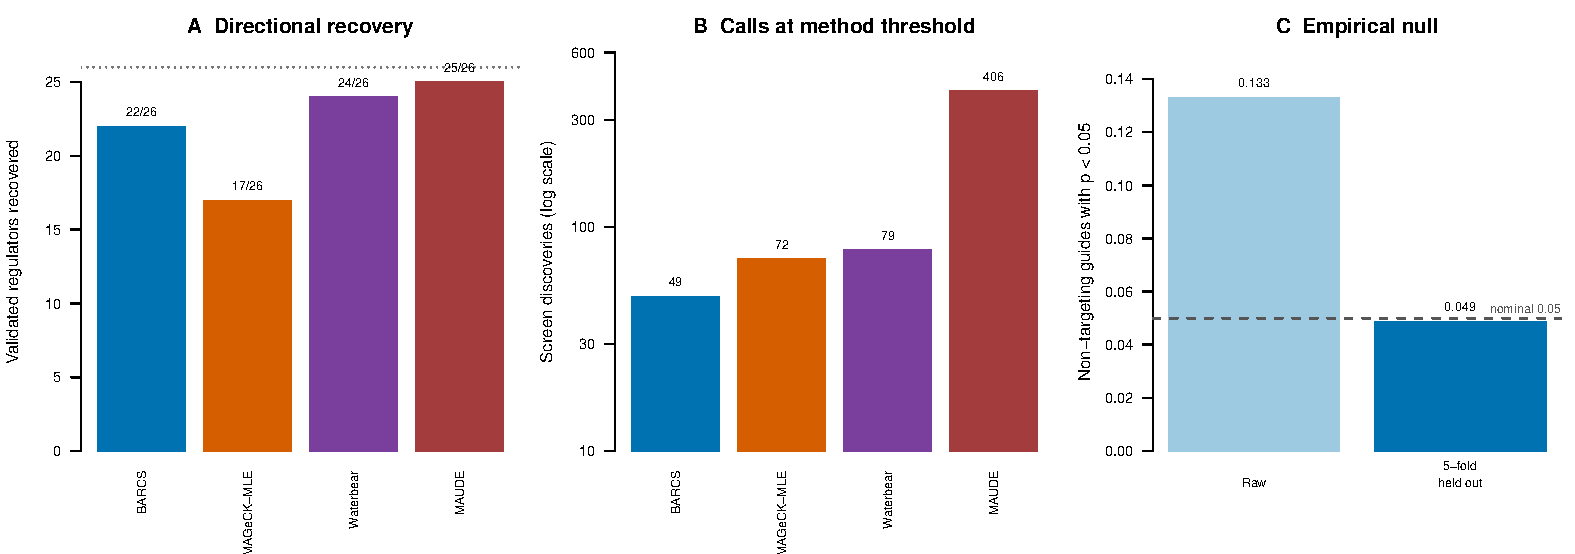
\includegraphics[width=\textwidth]{figures/waterbear_facs_main.pdf}
\caption{\textbf{Supporting ordered-bin IL2RA benchmark.}  (A) Directional
recovery of 26 independently validated regulators.  (B) Total discoveries at
each method's threshold (log scale).  (C) Empirical non-targeting-guide
$p<0.05$ rate before and after BARCS control calibration; the dashed line is
the nominal rate.}
\label{fig:waterbear}
\end{figure}

\input{sections/results/supp_ht29-cnv}

\paragraph{Additional multivariable and endpoint benchmarks.}
The following analyses test backward compatibility, multivariable effect
concordance, copy-number sensitivity, and preprocessing contracts.  They are
reported separately because none is a direct test of the primary longitudinal
generalization.

% !TeX root = ../../main.tex
\subsection{A multi-coefficient design on real data: GSE70038}

The benchmarks so far test one coefficient at a time.  GSE70038 is the case
where the design matrix earns its place: 64,747 guides in 16 libraries from two
glioblastoma stem-cell lines and two neural stem-cell lines, with duplicate
initial and terminal samples \citep{toledo2015pkmyt1}.  The scientific target is
four cell-line-specific terminal effects estimated \emph{jointly} against one
shared initial baseline.  Four separate two-group tests cannot express that: each
would re-estimate the baseline from its own pair, discarding the other twelve
libraries that inform it.  This is therefore not a continuous-phenotype
benchmark but the multivariable one, and it is the design MAGeCKFlute documents
as the canonical multi-condition layout.

We followed the design-matrix rules in Table~5 and Box~3 of the MAGeCKFlute
protocol \citep{wang2019mageckflute}.  The first column is one for every
library; each initial library has zeros elsewhere; and each terminal library
has one in exactly one of four cell-line columns.  The same $16\times5$ matrix
was supplied to beta-binomial regression and the official MAGeCK-MLE 0.5.9.5
executable.  MAGeCK used median normalization and its Wald inference.  For the
beta-binomial result, guide effects were summarized by their within-gene
median, and directional guide $p$-values were combined by Stouffer's method.
This aggregation is an explicit comparison device, not a proposed replacement
for MAGeCK's gene model.

The ``effect rank correlation'' reported below is calculated in this analysis,
not copied from GEO or the MAGeCKFlute paper.  Separately for each terminal
coefficient, we pair all genes available from both methods.  The
beta-binomial effect is the within-gene median guide coefficient, and the
MAGeCK effect is its official MLE beta.  We assign average ranks to these two
effect vectors and take their Pearson correlation, which is exactly Spearman's
rank correlation.  The 18,077 paired effects and their ranks for every
coefficient are included with the deposited analysis output.

\begin{table}[ht]
\centering
\caption{Effect concordance between \methodswatch{barcsblue} BARCS and
\methodswatch{mageckorange} official MAGeCK-MLE on GSE70038.  Jaccard is the
overlap divided by the union of the 200 most depleted genes from each method.
Higher agreement is better; column maxima are shown in bold.}
\label{tab:gse}
\begin{tabular}{lrr}
\toprule
Terminal coefficient & Spearman effect correlation & Top-200 Jaccard\\
\midrule
GSC0131 & \textbf{0.928} & 0.550\\
GSC0827 & 0.888 & 0.533\\
NSCCB660 & 0.905 & 0.544\\
NSCU5 & 0.915 & \textbf{0.562}\\
\bottomrule
\end{tabular}
\end{table}

Concordance here is the validation rather than the finding.  The comparison is
not circular: beta-binomial regression conditions on each library total, whereas
MAGeCK uses a normalized negative-binomial count model with guide-efficiency
estimation \citep{li2015mageckvispr}.  Two models that disagree on the noise
distribution, the normalization, and the guide-efficiency treatment nevertheless
place the four coefficient vectors in the same order, with all four effect
correlations above 0.88.  That is the evidence that the model-matrix interface
recovers the intended estimand on a real screen rather than a reparameterised
approximation of it.  These correlations
measure agreement of the inferred gene ordering; they are not likelihood,
calibration, or predictive-fit statistics and therefore cannot identify a
better-fitting method.  In GSC0131, the
published convergent dependency PKMYT1 has effect $-0.987$ and FDR
$1.87\times10^{-8}$ under beta-binomial regression, versus beta $-0.786$ and
Wald FDR $4.53\times10^{-8}$ under MAGeCK-MLE.  Both also recover HEATR1,
TFAP2C, and WEE1 depletion.  Figure~\ref{fig:gse} shows the complete GSC0131
comparison; the reproducible PDF contains one page per terminal coefficient.

\begin{figure}[ht]
\centering
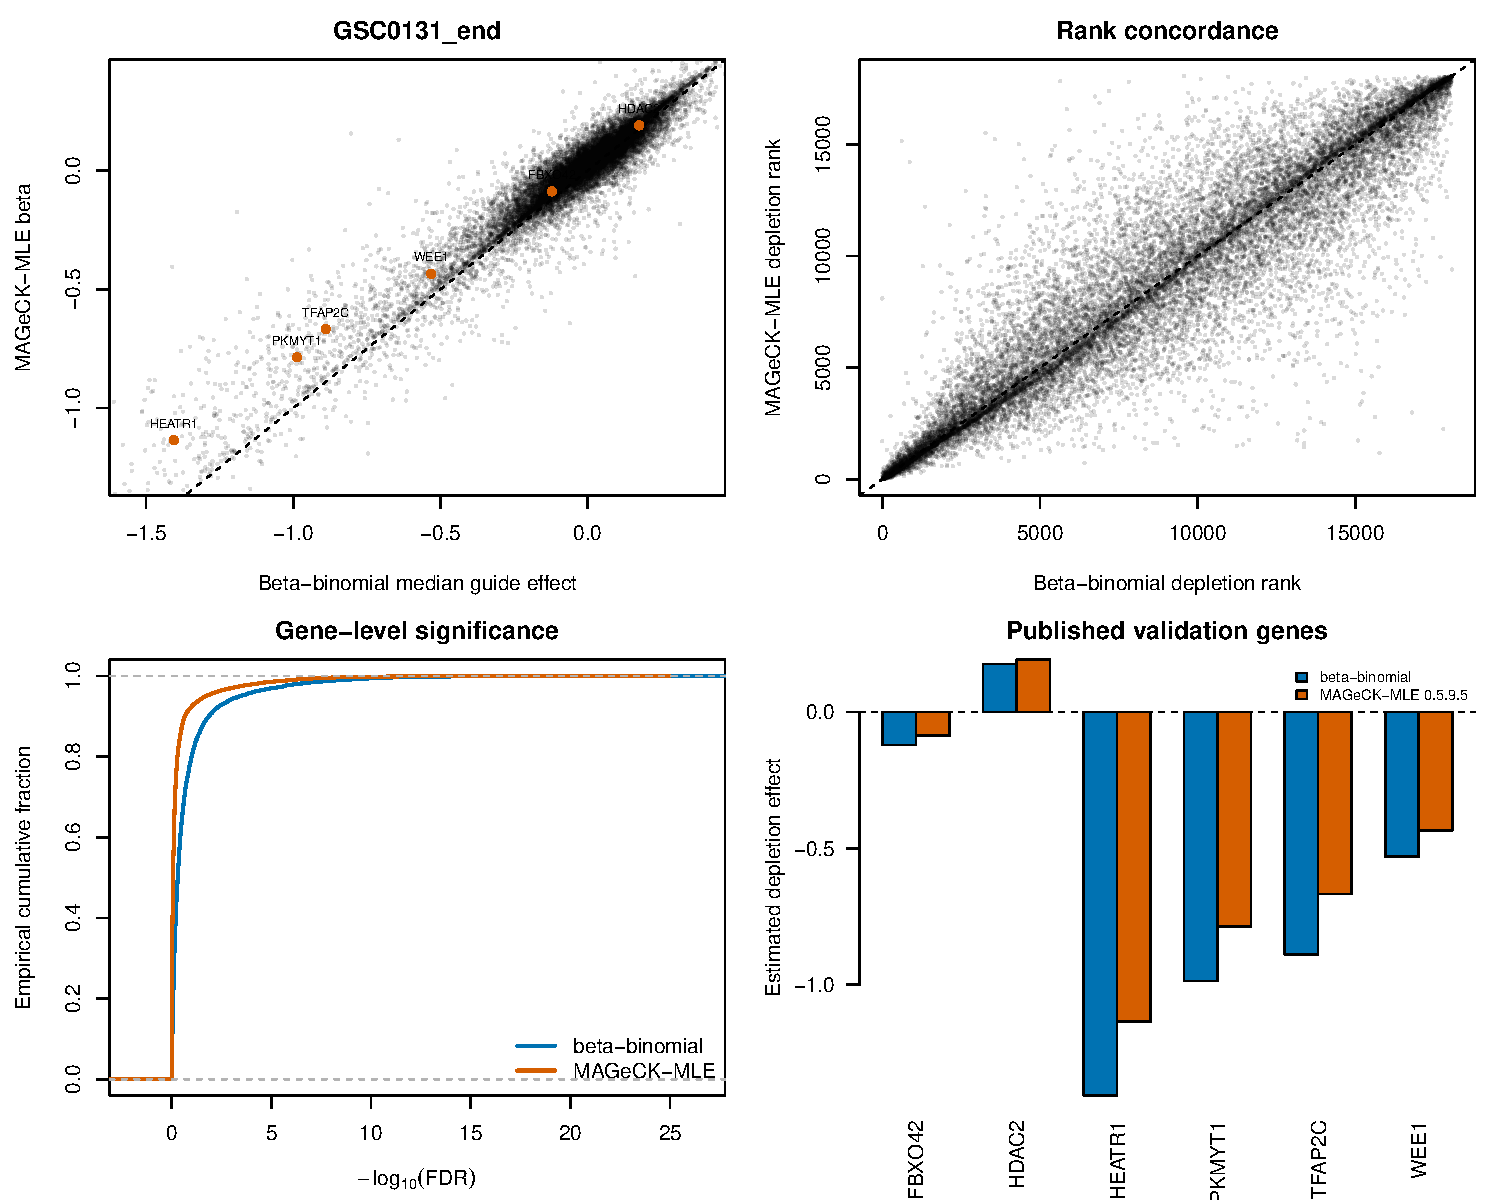
\includegraphics[width=\textwidth]{figures/gse70038_head_to_head.pdf}
\caption{GSE70038 GSC0131 head-to-head.  (A) Gene effects, with dark points
marking the prespecified genes PKMYT1, HEATR1, TFAP2C, FBXO42, HDAC2, and WEE1.
(B) Depletion-rank concordance.  (C) Gene-level FDR distributions.  (D)
Effects for the published validation genes.}
\label{fig:gse}
\end{figure}
\clearpage

% !TeX root = ../../main.tex
\subsection{Endpoint benchmark and copy-number audit}

To ask which method ranks biological dependencies better, we used the
Brunello A375 negative-selection screen of \citet{sanson2018optimized}, bundled
with CB\textsuperscript{2}.  This is an ordinary endpoint screen rather than a
continuous-phenotype experiment, but it supplies an external target unavailable
in GSE70038: reference essential genes should rank ahead of reference
nonessential genes \citep{hart2017evaluation}.  The beta-binomial score combines guide
evidence by directional Stouffer aggregation; the MAGeCK score uses the
official MLE beta and Wald $p$-value.  Both are oriented so larger scores mean
stronger depletion.

\subsubsection{Copy-number-aware analysis}

Copy number is a gene-level property of A375, not a sample-level covariate:
for a given guide it is constant across the plasmid and three terminal
libraries.  Adding it directly to the four-row sample design would therefore
be non-identifiable with the endpoint effect.  Instead, we downloaded the
A375 gene-level profile (ACH-000219) from DepMap Public 19Q3
\citep{depmap19q3,meyers2017cnv} and used MAGeCK 0.5.9.5's official
\texttt{--cnv-norm} piecewise correction.  For an apples-to-apples comparison,
the same MAGeCK piecewise normalizer was applied to the beta-binomial
within-gene median effects.  It adjusts effect sizes after model fitting; it
does not refit either count likelihood.  The common CNV-complete evaluation set
contains 1,506 essential and 869 nonessential genes.

\begin{table}[ht]
\centering
\caption{CNV-aware Sanson A375 benchmark.  The final column is Spearman
correlation between effect and copy number among reference nonessential genes;
values nearer zero indicate less residual CNV-associated depletion.  F1 uses
nominal FDR 0.05 and a negative effect.  Higher discrimination metrics and
CNV correlation closest to zero are highlighted.}
\label{tab:sanson}
\small
\setlength{\tabcolsep}{4pt}
\begin{tabular}{lrrrr}
\toprule
Method & AUROC & Avg. precision & F1 & CNV correlation\\
\midrule
\methodswatch{barcsblue} BARCS &
  \textcolor{barcsblue}{\textbf{0.9598}} & 0.9786 &
  \textcolor{barcsblue}{\textbf{0.8531}} & $-0.185$\\
\methodswatch{barcsblue} BARCS + CNV &
  0.9533 & 0.9762 & \textcolor{barcsblue}{\textbf{0.8531}} & $-0.042$\\
\methodswatch{mageckorange} Official MAGeCK-MLE &
  \textcolor{mageckorange}{\textbf{0.9598}} &
  \textcolor{mageckorange}{\textbf{0.9795}} &
  0.8277 & $-0.207$\\
\methodswatch{mageckorange} Official MAGeCK-MLE + CNV &
  0.9501 & 0.9762 & 0.8277 &
  \textcolor{mageckorange}{$\mathbf{-0.006}$}\\
\bottomrule
\end{tabular}
\end{table}

CNV correction substantially removes the intended nuisance association:
$-0.185$ to $-0.042$ for beta-binomial effects and $-0.207$ to $-0.006$ for
MAGeCK.  It does not improve essential-gene discrimination in this screen.
AUROC decreases by 0.0066 and 0.0097, respectively, and the 0.05-FDR calls are
unchanged.  This is not a contradiction: bias removal and gold-standard
classification are different targets, and amplified genes can include both
dependencies and nondependencies.

After CNV correction, beta-binomial versus MAGeCK global ranking remains
indistinguishable: the AUROC difference is 0.00316 (paired
stratified-bootstrap 95\% CI $-0.00265$ to $0.00924$), and the average
precision difference is effectively zero (95\% CI $-0.00349$ to $0.00295$).
At nominal FDR 0.05, beta-binomial retains 4.18 percentage points more recall
(95\% CI 2.66 to 5.71) and an F1 advantage of 0.0253 (95\% CI 0.0148 to
0.0362).

% !TeX root = ../../main.tex
\subsection{False-discovery conclusions depend on the analysis contract}
\label{sec:fdr-audit}

We audited a deposited Chronos benchmark that compared CB\textsuperscript{2},
MAGeCK, JACKS, DrugZ, and Chronos \citep{dempster2025fdr,
dempster2025fdrdata}.  The key issue was the beta-binomial denominator.  In
the reported null-only Avana analysis, the count matrix was restricted to
control genes before fitting, so its column sums no longer represented full
sequencing depth.  Reusing the full-library CB\textsuperscript{2} probabilities
for the same test genes changed the number of FDR 0.10 discoveries from 152 to
zero.

\begin{table}[htbp]
\centering
\caption{Data-driven audit of the external false-discovery benchmark.
``Known'' refers to the 28 literature-curated condition--gene combinations,
not a complete truth set.}
\label{tab:chronosaudit}
\small
\setlength{\tabcolsep}{4pt}
\begin{tabular}{p{0.18\textwidth}p{0.17\textwidth}p{0.15\textwidth}
                p{0.16\textwidth}p{0.20\textwidth}}
\toprule
Audit & Reference set & Reported result & Full-total reanalysis &
Additional diagnostic\\
\midrule
Avana null-only &
Null genes, five cell lines &
152 calls at FDR 0.10 &
0 calls at FDR 0.10 &
Largest null $p<0.05$ rate: 0.145\\
PSN1 two-versus-two split &
Null pseudo-condition &
0 gene calls &
0 gene calls &
Guide $p<0.05$: 0.0481 raw, 0.0465 scaled\\
DeWeirdt differential screens &
28 curated interactions &
0/28 known recovered &
38 calls; 1/28 known recovered &
37/38 calls arose in one comparison\\
\bottomrule
\end{tabular}
\end{table}

The PSN1 result shows that pooling one guide dispersion across the design can
avoid the extreme loss of power produced by separate two-replicate variance
estimates while retaining a near-nominal guide null.  The DeWeirdt result shows
the boundary of that improvement: BARCS recovered only MCL1 under A-1331852,
and nearly all other calls came from one OVCAR8--olaparib comparison without
recovering BRCA1 or BRCA2.  A global treatment-associated quality shift cannot
be separated from treatment with only two replicates per arm.

These results do not establish a winner against a complete ground truth.
They show that pre-fit guide subsetting and common normalization can alter the
effective depth seen by a library-total-conditional model.  Comparator studies
must preserve full-library totals, separate calibration guides from evaluation
guides, and use blocked permutations or independent validation for
differential screens.



\end{document}
